% Options for packages loaded elsewhere
\PassOptionsToPackage{unicode}{hyperref}
\PassOptionsToPackage{hyphens}{url}
%
\documentclass[
]{article}
\usepackage{amsmath,amssymb}
\usepackage{lmodern}
\usepackage{iftex}
\ifPDFTeX
  \usepackage[T1]{fontenc}
  \usepackage[utf8]{inputenc}
  \usepackage{textcomp} % provide euro and other symbols
\else % if luatex or xetex
  \usepackage{unicode-math}
  \defaultfontfeatures{Scale=MatchLowercase}
  \defaultfontfeatures[\rmfamily]{Ligatures=TeX,Scale=1}
\fi
% Use upquote if available, for straight quotes in verbatim environments
\IfFileExists{upquote.sty}{\usepackage{upquote}}{}
\IfFileExists{microtype.sty}{% use microtype if available
  \usepackage[]{microtype}
  \UseMicrotypeSet[protrusion]{basicmath} % disable protrusion for tt fonts
}{}
\makeatletter
\@ifundefined{KOMAClassName}{% if non-KOMA class
  \IfFileExists{parskip.sty}{%
    \usepackage{parskip}
  }{% else
    \setlength{\parindent}{0pt}
    \setlength{\parskip}{6pt plus 2pt minus 1pt}}
}{% if KOMA class
  \KOMAoptions{parskip=half}}
\makeatother
\usepackage{xcolor}
\IfFileExists{xurl.sty}{\usepackage{xurl}}{} % add URL line breaks if available
\IfFileExists{bookmark.sty}{\usepackage{bookmark}}{\usepackage{hyperref}}
\hypersetup{
  hidelinks,
  pdfcreator={LaTeX via pandoc}}
\urlstyle{same} % disable monospaced font for URLs
\usepackage{longtable,booktabs,array}
\usepackage{calc} % for calculating minipage widths
% Correct order of tables after \paragraph or \subparagraph
\usepackage{etoolbox}
\makeatletter
\patchcmd\longtable{\par}{\if@noskipsec\mbox{}\fi\par}{}{}
\makeatother
% Allow footnotes in longtable head/foot
\IfFileExists{footnotehyper.sty}{\usepackage{footnotehyper}}{\usepackage{footnote}}
\makesavenoteenv{longtable}
\usepackage{graphicx}
\makeatletter
\def\maxwidth{\ifdim\Gin@nat@width>\linewidth\linewidth\else\Gin@nat@width\fi}
\def\maxheight{\ifdim\Gin@nat@height>\textheight\textheight\else\Gin@nat@height\fi}
\makeatother
% Scale images if necessary, so that they will not overflow the page
% margins by default, and it is still possible to overwrite the defaults
% using explicit options in \includegraphics[width, height, ...]{}
\setkeys{Gin}{width=\maxwidth,height=\maxheight,keepaspectratio}
% Set default figure placement to htbp
\makeatletter
\def\fps@figure{htbp}
\makeatother
\setlength{\emergencystretch}{3em} % prevent overfull lines
\providecommand{\tightlist}{%
  \setlength{\itemsep}{0pt}\setlength{\parskip}{0pt}}
\setcounter{secnumdepth}{-\maxdimen} % remove section numbering
\ifLuaTeX
  \usepackage{selnolig}  % disable illegal ligatures
\fi

\author{}
\date{}

\begin{document}

{
\setcounter{tocdepth}{2}
\tableofcontents
}
\hypertarget{extended-literature-review-and-research-methodology-development}{%
\section{Extended Literature Review and Research Methodology
Development}\label{extended-literature-review-and-research-methodology-development}}

\textbf{Phase 2 --- Data Analysis and Visualization}

\textbf{Project:} Explainable Visualization and Monitoring of Machine
Learning Data Drift in Dynamic Environments

\textbf{Authors:} Saneedullah and Ahmed Bilal

\textbf{Date:} October 2026

\begin{center}\rule{0.5\linewidth}{0.5pt}\end{center}

\hypertarget{abstract}{%
\subsection{Abstract}\label{abstract}}

Phase 1 established that concept-drift detection, feature-level
explanation, and predictive adaptation are often studied separately, and
that a detected input change does not by itself establish material model
harm. Phase 2 extends that review with eight additional peer-reviewed
studies published in 2025--2026 and develops a technically justified
methodology for evaluating evidence reliability in explainable
data-drift monitoring. The review compares detection benchmarks,
window-dependent interpretation, label-based uncertainty, label-free
batching, causal explanation, explanation-triggered retraining,
recurrent conformal monitoring, and performative feedback. A focused
three-paper synthesis identifies three gaps: detection is not harm;
reference windows change what is being tested; and delayed labels limit
decision coverage. The proposed methodology freezes tabular classifiers,
separates input evidence from released-label loss evidence, and compares
fixed versus rolling input references under matched cohorts, label
delays, and assessment checkpoints. Independent synthetic streams
provide bounded risk truth; dependent controls and natural case studies
test robustness and descriptive transfer. The contribution is an
evaluation framework and an evidence-separated visualization design, not
a new detector, an implemented system, or a claim of deployment benefit.

\begin{center}\rule{0.5\linewidth}{0.5pt}\end{center}

\hypertarget{introduction-and-continuity-with-phase-1}{%
\subsection{1. Introduction and Continuity with Phase
1}\label{introduction-and-continuity-with-phase-1}}

\hypertarget{what-phase-1-established}{%
\subsubsection{1.1 What Phase 1
established}\label{what-phase-1-established}}

The Phase 1 review examined ten studies spanning representation-based
detection, feature-level monitoring, proactive adaptation, shift
identification, and visual analytics. Its central finding was that the
literature contains many ways to detect or describe change, but few
controlled comparisons of whether monitoring evidence supports a correct
statement about model harm. Four conclusions carry into Phase 2.

First, detection scores are not harm measures. DriftLens compares
Gaussian summaries of deep representations and reports strong detection
performance, but its severity--distance correlation measures injected
change rather than predictive loss (Greco et al., 2025). DDE estimates
feature drift from observed alarms and co-drift relationships, but its
targets are detector-derived rather than independently certified feature
events (Szűcs \& Németh, 2025).

Second, reference and window choices change the question being answered.
A fixed reference asks whether the current cohort differs from a
historical population; a rolling reference asks whether it differs from
the recent past. These are different targets, and an alarm under one is
not automatically an alarm under the other.

Third, label access determines what can be claimed.
Prediction-uncertainty methods may appear label-free, but the true-class
uncertainty score used by PUDD requires released labels (Lu et al.,
2025). Adaptive methods such as proactive Hoeffding trees and ADWIN-U
also depend on labelled feedback or update policies (Guerrero Cano et
al., 2026; Assis \& Souza, 2025).

Fourth, visualization and explanation are established as useful
interfaces, but their decision benefit is not established. DriftVis and
ConceptExplorer coordinate detection, feature, and prediction views, yet
their case studies do not isolate the effect of the interface on
decision quality (Yang et al., 2020; Wang et al., 2020).
Parallel-histogram displays such as PHT offer a complementary view of
feature distributions over time, but their marginal views can miss
interaction-only change (Gălmeanu \& Andonie, 2024).

Phase 1 translated these findings into three main gaps: the decision
benefit of unified detection, localization, and visual explanation; the
relation between statistical drift magnitude and model degradation; and
interpretability and external validity in complex image domains. It also
identified supporting gaps in calibration, observability, label delay,
and pipeline costs. Supporting Phase 1 sources---including the
benchmarking critique of Souza et al.~(2020), the performance-aware
overview of Bayram et al.~(2022), the explanation studies of Hinder et
al.~(2023, 2024), the image-stream survey of Tran et al.~(2026), the
medical shift study of Roschewitz et al.~(2025), the process-drift study
of Kraus and van der Aa (2025), and the unsupervised-detector benchmark
of Lukats et al.~(2025)---provide background and are not counted among
the eight additional selections.

\hypertarget{scope-refinement-for-phase-2}{%
\subsubsection{1.2 Scope refinement for Phase
2}\label{scope-refinement-for-phase-2}}

Phase 2 selects the second Phase 1 gap---the relation between monitoring
evidence and predictive harm---and narrows it to a controlled
tabular-classification study. This scope decision is deliberate.

\begin{itemize}
\tightlist
\item
  \textbf{Independent truth is available.} Synthetic generators can
  define the pre-change population, the changed population, and the
  expected error risk of a frozen classifier. This permits evaluation of
  whether an alarm corresponds to material harm, rather than assuming
  that a detected change is harmful.
\item
  \textbf{The classifier can be frozen.} Freezing the model separates
  monitoring evidence from adaptation. A change in accuracy after an
  update confounds the detector with the learning policy; a frozen
  classifier removes that confound.
\item
  \textbf{Reference policy can be manipulated.} Fixed and rolling input
  references can be applied to the same realised stream, so their effect
  on alarm interpretation can be compared directly.
\item
  \textbf{Label delay can be controlled.} The release time of each label
  can be declared, allowing the study to distinguish evidence
  availability from evidence correctness.
\item
  \textbf{The study is feasible.} A tabular design with public datasets
  and a small number of classifiers can be completed within a course
  project, whereas image-domain transfer and human-subject evaluation
  would require separate studies.
\end{itemize}

The scope therefore excludes image representations, adaptive retraining,
causal discovery, and analyst decision benefit. These are not dismissed;
they are deferred because each requires a different design, dataset, and
ethical or computational budget. The Phase 2 contribution is an
evaluation framework and an evidence-separated visualization design, not
a new detector or a deployed monitoring system.

\hypertarget{contributions-and-roadmap}{%
\subsubsection{1.3 Contributions and
roadmap}\label{contributions-and-roadmap}}

This submission makes five contributions:

\begin{enumerate}
\def\labelenumi{\arabic{enumi}.}
\tightlist
\item
  It extends the Phase 1 corpus with eight additional 2025--2026 studies
  and audits their eligibility.
\item
  It synthesises the eight studies around evaluation target, label
  access, reference policy, and generalisation.
\item
  It provides a focused nine-column comparison of three representative
  studies.
\item
  It refines three research gaps and answers the six justification
  questions explicitly.
\item
  It specifies a twelve-step methodology, a matched experimental design,
  an evaluation plan, and two methodology diagrams.
\end{enumerate}

The remainder of the document follows the four required deliverables.
Section 2 presents the extended literature review. Section 3 refines the
research gap and states the research question. Section 4 develops the
twelve-step methodology, including the visualization design. Section 5
presents the methodology diagrams. Section 6 discusses reproducibility,
ethics, and risk. Section 7 concludes. The appendices provide a
compliance checklist and venue-eligibility notes.

\begin{quote}
\textbf{Scope and claims.} All project activities in this document are
proposed. Published findings are attributed to their sources. No model
implementation, completed experiment, measured project result, analyst
benefit, or adaptation benefit is claimed.
\end{quote}

\begin{center}\rule{0.5\linewidth}{0.5pt}\end{center}

\hypertarget{deliverable-1-extended-literature-review}{%
\subsection{2. Deliverable 1 --- Extended Literature
Review}\label{deliverable-1-extended-literature-review}}

\hypertarget{selection-protocol}{%
\subsubsection{2.1 Selection protocol}\label{selection-protocol}}

The Phase 1 corpus remains the foundation of the review. The Phase 2
corpus adds eight studies, labelled S1--S8, that were not part of the
Phase 1 bibliography. Selection followed six criteria:

\begin{itemize}
\tightlist
\item
  \textbf{Date:} published in 2025 or 2026. Publication year refers to
  the archival proceedings or chapter, not an earlier preprint.
\item
  \textbf{Type:} original research article, conference paper, or
  research chapter. Editorials, opinions, news items, general webpages,
  and stand-alone preprints were excluded.
\item
  \textbf{Venue:} peer-reviewed archival venue from ACM, IEEE, AAAI,
  Springer, or PMLR. The brief permits Q1--Q2 journals, conference
  papers, and book chapters; the eight additions use the
  conference-paper and book-chapter routes.
\item
  \textbf{Relevance:} directly concerned with drift detection, drift
  explanation, monitoring under label constraints, recurrence, or
  adaptation.
\item
  \textbf{Method:} an identifiable dataset or data source, method, and
  evaluation.
\item
  \textbf{Access:} full text available for critical review, with
  publication metadata verifiable.
\end{itemize}

The eight studies are a purposive set, not a systematic sample of all
drift research. They were chosen to cover the evidence chain from
detection to explanation to action. This is appropriate for a
methodology-development phase, but it limits any claim of exhaustive
coverage.

\textbf{Table 1. Additional paper selection and eligibility audit.}

\begin{longtable}[]{@{}
  >{\raggedright\arraybackslash}p{(\columnwidth - 12\tabcolsep) * \real{0.14}}
  >{\raggedright\arraybackslash}p{(\columnwidth - 12\tabcolsep) * \real{0.14}}
  >{\raggedright\arraybackslash}p{(\columnwidth - 12\tabcolsep) * \real{0.14}}
  >{\raggedright\arraybackslash}p{(\columnwidth - 12\tabcolsep) * \real{0.14}}
  >{\raggedright\arraybackslash}p{(\columnwidth - 12\tabcolsep) * \real{0.14}}
  >{\raggedright\arraybackslash}p{(\columnwidth - 12\tabcolsep) * \real{0.14}}
  >{\raggedright\arraybackslash}p{(\columnwidth - 12\tabcolsep) * \real{0.14}}@{}}
\toprule
ID & Study & Year & Venue & Type & Publisher & Eligibility route \\
\midrule
\endhead
S1 & Cerqueira et al., \emph{A Framework for Evaluating and Benchmarking
Concept Drift Detection Methods} & 2026 & ACM SIGKDD Conference (KDD) &
Conference paper & ACM & Full archival conference paper \\
S2 & Gower-Winter et al., \emph{The Window Dilemma: Why Concept Drift
Detection is Ill-Posed} & 2026 & Advances in Intelligent Data Analysis
(IDA), LNCS & Research chapter & Springer Nature & Peer-reviewed book
chapter \\
S3 & Lu et al., \emph{Early Concept Drift Detection via Prediction
Uncertainty} & 2025 & AAAI Conference on Artificial Intelligence &
Conference paper & AAAI & Full archival conference paper \\
S4 & Tan et al., \emph{Flexible and Efficient Drift Detection Without
Labels} & 2025 & IEEE International Conference on Data Mining Workshops
(ICDMW) & Workshop paper & IEEE & Peer-reviewed conference paper \\
S5 & Komnick et al., \emph{Causal Explanation of Concept Drift---A Truly
Actionable Approach} & 2026 & ECML PKDD 2025 Workshops, CCIS & Research
chapter & Springer Nature & Peer-reviewed book chapter \\
S6 & Teixeira et al., \emph{Detecting Concept Drift with SHapley
Additive ExPlanations for Intelligent Model Retraining in Energy
Generation Forecasting} & 2025 & xAI Conference, CCIS & Research chapter
& Springer Nature & Peer-reviewed book chapter \\
S7 & Eliades \& Papadopoulos, \emph{A Conformal Martingales Approach for
Recurrent Concept Drift} & 2025 & COPA 2025, PMLR & Conference paper &
PMLR & Peer-reviewed conference paper \\
S8 & Gower-Winter et al., \emph{Identifying Predictions That Influence
the Future: Detecting Performative Concept Drift in Data Streams} & 2025
& AAAI Conference on Artificial Intelligence & Conference paper & AAAI &
Full archival conference paper \\
\bottomrule
\end{longtable}

The three focal studies are S1--S3. They are complementary rather than
interchangeable: S1 evaluates whether detectors recover controlled
change events, S2 shows that the window definition changes what
detection means, and S3 evaluates a prediction-uncertainty signal that
depends on released labels. Together they isolate the three issues that
motivate the proposed study: detection truth, reference interpretation,
and label access.

\hypertarget{critical-review-of-the-eight-additional-studies}{%
\subsubsection{2.2 Critical review of the eight additional
studies}\label{critical-review-of-the-eight-additional-studies}}

The eight studies fall into two groups. S1--S4 examine detection
evaluation, window choice, label dependence, and computational budgets.
S5--S8 examine explanation, recurrence, retraining, and feedback. The
distinction matters because the later group often changes the model or
the data-generating process, whereas the proposed study holds both
fixed.

\textbf{Table 2. Critical review of the eight additional studies.}

\begin{longtable}[]{@{}
  >{\raggedright\arraybackslash}p{(\columnwidth - 8\tabcolsep) * \real{0.20}}
  >{\raggedright\arraybackslash}p{(\columnwidth - 8\tabcolsep) * \real{0.20}}
  >{\raggedright\arraybackslash}p{(\columnwidth - 8\tabcolsep) * \real{0.20}}
  >{\raggedright\arraybackslash}p{(\columnwidth - 8\tabcolsep) * \real{0.20}}
  >{\raggedright\arraybackslash}p{(\columnwidth - 8\tabcolsep) * \real{0.20}}@{}}
\toprule
ID & Data and method & Main findings & Author-stated limitations &
Reviewer-identified limitations \\
\midrule
\endhead
S1 & Seven public stream datasets (Asfault, Electricity, Covertype,
GasSensorArray, NOAA, Posture, Rialto); controlled class-prior,
label-swap, permutation, and filtering transformations; 14 detectors; 50
Monte Carlo trials per dataset and drift type; leave-one-dataset-out
tuning. & Timing-aware metrics separate detector success from retraining
accuracy. SEED and STEPD are competitive across mechanisms; ABCD has
favourable false-alarm ranks. & Immediate post-prediction feedback;
temporal structure removed; four drift types; shuffled source order. &
Known input events do not establish correct excess-risk verdicts under
delayed labels. The benchmark evaluates event recovery, not the decision
value of an alarm. \\
S2 & Eleven binary and multiclass streams (including Electricity,
Covertype, Insects, NOAA, Rialto); time-ordered prequential evaluation;
explicit training, window, and reset schedules; DDM, ADWIN, D3, and IBDD
with naive Bayes, trees, and adaptive, incremental, resetting, or static
forests. & Accuracy and kappa show that the learning strategy matters,
not only drift awareness. ARF has median rank 2; AMF and incremental RF
rank 3; resetting RF rank 4. & Sampled windows need not represent
endpoint concepts; natural changes cannot all be verified; warm and cold
starts differ. & Classifier and adaptation comparisons do not isolate
matched cohort-risk decisions. The result is about predictive
performance under a window policy, not about the correctness of a harm
declaration. \\
S3 & Airline, Electricity, PowerSupply; Sine, Mixed, SEA variants;
CIFAR-10-CD; true-class prediction-uncertainty scores; adaptive
histograms and window cuts; chi-square testing; DNN, GNB, and VFDT
baselines. & PUDD ranks first in 17/24 incremental classic-detector
comparisons and in the top three in 20/24. & Manual thresholds;
guarantees concern individual window-pair tests; adaptive bucketing
choices. & The score uses the probability of the true class, so it
requires released labels. Sensitivity is not certification that excess
risk exceeds a material margin. \\
S4 & Gaussian mean, variance, and covariance simulations; batched
distances including MMD; paired tests; false-positive and false-negative
rates under computational budgets. & Batching can improve the
power--runtime trade-off in selected settings. & Independence of batch
triplets; simulation-based evaluation; selected distance families. &
Simulation power does not certify predictive harm on natural streams.
The method answers whether distributions differ, not whether the
classifier is harmed. \\
S5 & Semi-synthetic Adult and Portuguese Student Performance data;
modified Bayesian networks; PC causal discovery with a g-square test;
ten runs per scenario. & Graph orientation and identified drift features
are assessed; occupation is linked to time in 9/10 Adult Women in STEM
runs. & Global causal graph; discovery assumptions; limited scenarios. &
A global causal graph restricts transfer, and marginal ranking is a
weaker explanation object than a validated causal claim. The method
explains a constructed mechanism, not a deployment. \\
S6 & Porto photovoltaic and weather data from 2023 at 10-minute
intervals; 12 inputs; XGBoost regression; SHAP reference monitoring;
retraining trigger. & SHAP monitoring reaches RMSE 0.0879 versus 0.1089
for a fixed model, with 717 versus zero retrainings. & Single site;
tuning period overlaps the reported evaluation period; regression task.
& The improvement combines detection with the retraining policy, so it
does not isolate the value of the explanation. A single-site forecasting
result does not establish delayed classification-verdict reliability. \\
S7 & STAGGER, Electricity, and Airlines; inductive conformal
martingales; a pool of recurrent models; accuracy, detection delay,
false alarms, and model reuse. & Recurrence can be monitored with
conformal martingales; model reuse trades accuracy for reduced training.
& Nonconformity uses observed true labels; natural event truth is
incomplete; pool design choices. & The method requires labels and a
model pool. It evaluates recurrence detection and reuse, not whether a
frozen classifier's current cohort is materially harmed. \\
S8 & Synthetic feedback streams and semi-synthetic Water Potability,
Loan Status, and Credit Card data; CheckerBoard prediction
interventions. & Detection succeeds on Water Potability and Loan Status
in most settings but fails on the heavily imbalanced Credit Card case. &
Deliberate prediction interventions; self-fulfilling feedback; class
imbalance. & The design requires the monitor to influence the future,
which a frozen observational monitor cannot do. Transfer to passive
monitoring is therefore limited. \\
\bottomrule
\end{longtable}

Three patterns emerge. First, the strongest empirical studies evaluate a
clearly defined target: an injected event, a predictive accuracy
trajectory, a feature set, or a recurrence signal. None evaluates the
joint target of this proposal---a cohort-specific excess-risk verdict
under a fixed classifier, a chosen reference policy, and a declared
label delay. Second, label access is rarely treated as an experimental
factor. S1 assumes immediate feedback, S3 and S7 require true labels,
and S4 is label-free but evaluates a distributional distance rather than
harm. Third, the explanation and adaptation studies change the model or
the data-generating mechanism. S5 constructs a causal graph, S6 retrains
a forecaster, and S8 intervenes on predictions. Their findings are
relevant, but they cannot be pooled with a frozen-classifier monitoring
study as if they measured the same outcome.

\hypertarget{cross-paper-synthesis}{%
\subsubsection{2.3 Cross-paper synthesis}\label{cross-paper-synthesis}}

\textbf{Table 3. Evidence map across the eight additional studies.}

\begin{longtable}[]{@{}
  >{\raggedright\arraybackslash}p{(\columnwidth - 8\tabcolsep) * \real{0.20}}
  >{\raggedright\arraybackslash}p{(\columnwidth - 8\tabcolsep) * \real{0.20}}
  >{\raggedright\arraybackslash}p{(\columnwidth - 8\tabcolsep) * \real{0.20}}
  >{\raggedright\arraybackslash}p{(\columnwidth - 8\tabcolsep) * \real{0.20}}
  >{\raggedright\arraybackslash}p{(\columnwidth - 8\tabcolsep) * \real{0.20}}@{}}
\toprule
Study & Evaluation target & Label access & Reference or window & Main
limitation for the proposed study \\
\midrule
\endhead
S1 & Recovery and timing of controlled change events & Immediate
post-prediction feedback & Controlled transformations of source streams
& Event truth is not harm truth; delayed labels are absent. \\
S2 & Predictive accuracy and kappa under window and learning policies &
Labels used in prequential evaluation & Explicit training, window, and
reset schedules & Adaptation is confounded with monitoring. \\
S3 & Prediction-uncertainty ranking & True-class labels required &
Adaptive histograms and window cuts & Sensitivity is not a material-risk
certification. \\
S4 & Distributional difference under compute budgets & Label-free &
Batched reference and current samples & Simulation power is not
predictive harm. \\
S5 & Causal graph orientation and drift-feature identification & Labels
for the supervised task; causal assumptions & Global causal graph &
Constructed mechanism; limited transfer. \\
S6 & Forecasting error and retraining count & Labels for regression;
SHAP reference & Fixed reference and retraining trigger & Detection and
adaptation are combined. \\
S7 & Recurrence detection, delay, false alarms, model reuse & True
labels for nonconformity & Conformal martingale and model pool &
Requires labels and a model pool; not a frozen harm verdict. \\
S8 & Performative drift detection under interventions & Intervention
outcomes & CheckerBoard feedback streams & Requires prediction
interventions; passive monitoring cannot reproduce it. \\
\bottomrule
\end{longtable}

The synthesis yields four conclusions.

\textbf{Evaluation targets differ.} S1 asks whether a detector finds an
event; S2 asks how a window policy affects predictive performance; S3
asks whether an uncertainty signal ranks drift; S4 asks whether a
batched distance is efficient; S5 asks whether a causal graph is
oriented correctly; S6 asks whether a forecasting model improves after
retraining; S7 asks whether recurrence is detected and models can be
reused; S8 asks whether performative feedback is identifiable. These are
not interchangeable outcomes. A table that ranks them by a single score
would be misleading.

\textbf{Label access is a design variable, not a nuisance.} The
literature often assumes that labels arrive immediately or that a
true-class score is available. In deployment, labels may arrive after a
delay, only for a subset, or never. The proposed study treats label
release as an experimental factor because it changes which verdicts are
structurally possible.

\textbf{Reference policy changes the target.} S2 makes this explicit: a
sampled window need not represent the endpoint concept. S1 uses
controlled transformations against a source stream. S3 uses adaptive
windows. S4 batches observations. The proposed study therefore separates
the input reference from the predictive-risk reference: the input
reference can be fixed or rolling, while the harm target remains fixed.

\textbf{Explanation and action are separate claims.} S5 produces a
causal explanation under a graph, S6 uses SHAP to trigger retraining,
and S8 detects feedback caused by predictions. Each is valuable, but
none establishes that a marginal feature ranking is a causal explanation
or that a correct alarm implies a beneficial intervention. The proposed
study treats feature rankings as distributional screening evidence and
evaluates verdict correctness, not intervention benefit.

\hypertarget{three-paper-comparison}{%
\subsubsection{2.4 Three-paper
comparison}\label{three-paper-comparison}}

S1--S3 are selected for the focused comparison because their designs
isolate the three central issues. S1 provides controlled event truth and
timing-aware metrics. S2 shows that the window and learning policy
change the meaning of the comparison. S3 provides a label-dependent
uncertainty signal and evaluates it through classification and ranking.
The comparison is synthesised rather than copied: the rows below retain
each study's task, dataset, and evaluation conditions.

\textbf{Table 4. Synthesised comparison of three representative
studies.}

\begin{longtable}[]{@{}
  >{\raggedright\arraybackslash}p{(\columnwidth - 16\tabcolsep) * \real{0.11}}
  >{\raggedright\arraybackslash}p{(\columnwidth - 16\tabcolsep) * \real{0.11}}
  >{\raggedright\arraybackslash}p{(\columnwidth - 16\tabcolsep) * \real{0.11}}
  >{\raggedright\arraybackslash}p{(\columnwidth - 16\tabcolsep) * \real{0.11}}
  >{\raggedright\arraybackslash}p{(\columnwidth - 16\tabcolsep) * \real{0.11}}
  >{\raggedright\arraybackslash}p{(\columnwidth - 16\tabcolsep) * \real{0.11}}
  >{\raggedright\arraybackslash}p{(\columnwidth - 16\tabcolsep) * \real{0.11}}
  >{\raggedright\arraybackslash}p{(\columnwidth - 16\tabcolsep) * \real{0.11}}
  >{\raggedright\arraybackslash}p{(\columnwidth - 16\tabcolsep) * \real{0.11}}@{}}
\toprule
\# & Title & Year & Dataset used & Preprocessing & Models / techniques &
Evaluation metrics & Results & Limitations / research gap \\
\midrule
\endhead
1 & A Framework for Evaluating and Benchmarking Concept Drift Detection
Methods (S1) & 2026 & Asfault, Electricity, Covertype, GasSensorArray,
NOAA, Posture, Rialto & Shuffle source streams; inject class-prior,
label-swap, permutation, or filtering changes; abrupt and gradual
transitions & 14 detectors; Hoeffding-tree core; 50 trials per dataset
and drift type; leave-one-dataset-out tuning & Event precision, recall,
F1; normalized delay; alarm and false-alarm rate; runtime & SEED and
STEPD are competitive across mechanisms; ABCD has favourable false-alarm
ranks (Tables 1--2; Sec. 5.3) & Immediate feedback; temporal structure
removed; four drift types. Known input events do not establish correct
excess-risk verdicts under delayed labels. \\
2 & The Window Dilemma: Why Concept Drift Detection is Ill-Posed (S2) &
2026 & Eleven binary and multiclass streams, including Electricity,
Covertype, Insects, NOAA, and Rialto & Time-ordered prequential
evaluation; explicit training, window, and reset schedules; warm and
cold starts & DDM, ADWIN, D3, IBDD; naive Bayes and trees; adaptive,
incremental, resetting, and static forests & Mean accuracy; kappa;
median algorithm rank & ARF median rank 2; AMF and incremental RF rank
3; resetting RF rank 4 (Table 1) & Sampled windows need not represent
endpoint concepts; natural changes cannot all be verified. Adaptation is
confounded with monitoring. \\
3 & Early Concept Drift Detection via Prediction Uncertainty (S3) & 2025
& Airline, Electricity, PowerSupply; Sine, Mixed, SEA variants;
CIFAR-10-CD & True-class prediction-uncertainty scores; adaptive
histograms and window cuts; Markov class-interest simulation for images
& PUDD; chi-square testing; DNN, GNB, VFDT; classic and adaptive
baselines & Prediction accuracy; average ranks; threshold and bucketing
sensitivity & First rank in 17/24 incremental classic-detector
comparisons; top three in 20/24 & Manual thresholds; guarantees concern
individual window-pair tests. The true-class score requires labels;
sensitivity is not certification of material excess risk. \\
\bottomrule
\end{longtable}

The three studies answer different questions. S1 evaluates the recovery
and timing of controlled change events. S2 compares the predictive
consequences of window and learning strategies. S3 evaluates a
true-class uncertainty signal through classification and ranking. Their
reported ranks and accuracies therefore remain attached to their
original tasks, datasets, and label assumptions. The research
opportunity follows from this difference in evaluation targets, not from
assuming that one reported score is directly better than another.

\hypertarget{implications-for-the-proposed-study}{%
\subsubsection{2.5 Implications for the proposed
study}\label{implications-for-the-proposed-study}}

The review yields six design requirements:

\begin{enumerate}
\def\labelenumi{\arabic{enumi}.}
\tightlist
\item
  \textbf{Use independent truth.} Detector output cannot serve as the
  ground truth for whether harm occurred. Synthetic generators must
  define the pre-change and changed populations, and an evaluator-only
  risk estimate must be kept separate from the monitor.
\item
  \textbf{Freeze the classifier.} Monitoring evidence must be evaluated
  without confounding it with retraining or adaptation.
\item
  \textbf{Treat reference policy as a factor.} Fixed and rolling input
  references must be compared on the same realised stream, with one
  common predictive-risk reference.
\item
  \textbf{Model label delay explicitly.} Prediction time, label-release
  time, and assessment checkpoint must be separate fields.
\item
  \textbf{Evaluate verdict correctness and coverage.} A detector that
  never decides has low error but no decision value; a detector that
  always decides may make unsupported claims. Both coverage and error
  are required.
\item
  \textbf{Display evidence status.} A monitoring interface should show
  what is known, what is delayed, and what remains uncertain. It should
  not present an input alarm as proof of harm or a feature ranking as a
  causal explanation.
\end{enumerate}

\begin{center}\rule{0.5\linewidth}{0.5pt}\end{center}

\hypertarget{deliverable-2-refined-research-gap}{%
\subsection{3. Deliverable 2 --- Refined Research
Gap}\label{deliverable-2-refined-research-gap}}

\hypertarget{gap-synthesis-matrix}{%
\subsubsection{3.1 Gap synthesis matrix}\label{gap-synthesis-matrix}}

The three gaps below are joint limitations of S1--S3, cross-checked
against S4--S8. They do not claim that delayed monitoring, window
effects, or explanation integration are absent from prior research. They
identify a specific combination that the reviewed protocols do not
isolate.

\textbf{Table 5. Research gap synthesis based on the three focal
papers.}

\begin{longtable}[]{@{}
  >{\raggedright\arraybackslash}p{(\columnwidth - 8\tabcolsep) * \real{0.20}}
  >{\raggedright\arraybackslash}p{(\columnwidth - 8\tabcolsep) * \real{0.20}}
  >{\raggedright\arraybackslash}p{(\columnwidth - 8\tabcolsep) * \real{0.20}}
  >{\raggedright\arraybackslash}p{(\columnwidth - 8\tabcolsep) * \real{0.20}}
  >{\raggedright\arraybackslash}p{(\columnwidth - 8\tabcolsep) * \real{0.20}}@{}}
\toprule
Research gap & Evidence from S1 & Evidence from S2 & Evidence from S3 &
Proposed research opportunity \\
\midrule
\endhead
\textbf{G1. Detection is not material harm} & S1 measures event
detection and timing against controlled input changes. It does not
produce an uncertainty-qualified excess-risk verdict. & S2 shows that
accuracy and kappa depend on the window and learning strategy. Drift
awareness is not separated from adaptation. & S3 shows that
prediction-uncertainty sensitivity does not certify a material risk
margin. Its true-class score requires labels. & Freeze the classifier
and the risk target; compare proxy and verified verdict correctness
against independent expected-risk truth. \\
\textbf{G2. Reference policy changes the target} & S1 uses transformed
source streams as a common benchmark. It does not compare fixed and
rolling references against one harm truth. & S2 establishes that
window-dependent meaning is intrinsic to the detection problem. & S3
uses adaptive windowing, which changes which samples the detector
compares. & Define input and feature truth relative to the actual
population reference; retain one common harm truth across reference
policies. \\
\textbf{G3. Delayed evidence limits decision coverage} & S1 assumes
immediate post-prediction feedback, which simplifies the monitoring
workflow. & S2 shows that label-access regimes matter, but does not
isolate matched interval gating. & S3's true-class uncertainty score
cannot be computed before labels arrive. & Use named cohorts and fixed
checkpoints; quantify additional harm declarations, structural
unavailability, and deferral under identical interval rules. \\
\bottomrule
\end{longtable}

\textbf{G1: Detection is not harm.} S1 is a strong benchmark, but its
target is an input event. A detector can recover every injected change
and still fail to identify whether the frozen classifier's excess error
exceeds a material margin. S2 adds a second problem: if the window or
learning policy changes, an accuracy difference may reflect adaptation
rather than the monitoring signal. S3 adds a third: an uncertainty score
can be sensitive without being a calibrated harm probability. The
proposed study addresses the joint problem by holding the classifier and
risk target fixed and evaluating the verdict, not only the alarm.

\textbf{G2: Reference policy changes the target.} A fixed reference
compares the current cohort with a historical population. A rolling
reference compares it with the recent past. Both are legitimate, but
they answer different questions. S2 shows that the samples defining a
window can change what the detection problem means. S3's adaptive
windows make the same point operationally. The proposed study therefore
treats the input reference as an experimental factor and keeps the
predictive-risk reference fixed, so that differences in verdicts can be
attributed to the input reference rather than to a moving harm target.

\textbf{G3: Delayed evidence limits decision coverage.} S1 assumes
immediate feedback; S3 and S7 require true labels; S4 is label-free but
does not evaluate harm. In practice, labels arrive late, and a
monitoring policy may have to decide before they arrive. The proposed
study declares label-release times and assessment checkpoints. It
separates three reasons for not deciding: the labels are not yet
available, the interval crosses the harm margin, or the input alarm
gates a positive harm declaration. This distinction is necessary for
interpreting coverage.

\hypertarget{refinement-and-justification-of-the-research-gap}{%
\subsubsection{3.2 Refinement and justification of the research
gap}\label{refinement-and-justification-of-the-research-gap}}

\textbf{What has already been done.} Published research has established
controlled drift benchmarks, window-dependent interpretation,
uncertainty-based monitoring, feature-level explanation, recurrent model
selection, and feedback detection. Phase 1 reviewed representation-based
detection, selective feature monitoring, proactive adaptation, and
visual analytics. These are existing contributions on which the proposed
evaluation builds. The project does not claim to have implemented them.

\textbf{What approaches currently exist.} The literature contains five
families of monitoring evidence:

\begin{itemize}
\tightlist
\item
  \textbf{Label-free distributional detectors} such as KS, Wasserstein,
  Jensen--Shannon, and MMD. They can operate before labels arrive but
  answer whether distributions differ, not whether the classifier is
  harmed.
\item
  \textbf{Label-dependent error or uncertainty signals} such as
  released-label loss, true-class prediction uncertainty, and conformal
  nonconformity. They can be closer to harm but are unavailable before
  labels arrive.
\item
  \textbf{Adaptive-reference methods} that update windows or models in
  response to change. They can improve performance but confound
  monitoring with adaptation.
\item
  \textbf{Explanation-triggered methods} such as SHAP monitoring or
  causal graph analysis. They can describe what changed but introduce
  model or causal assumptions.
\item
  \textbf{Visual-analytics systems} that coordinate detection, features,
  and predictions. They can support interpretation but have not isolated
  decision benefit in controlled tasks.
\end{itemize}

\textbf{What the limitations are.} A detected input difference does not
imply a harmful loss change. An adaptive learner's accuracy also
reflects its update policy. Window boundaries affect the population
comparison. True-class scores cannot be computed before labels arrive.
Delayed and partially labelled streams have been surveyed by Alencar et
al.~(2026), but the reviewed protocols do not isolate the specific
matched-coverage comparison proposed here. Explanation fidelity, drift
sensitivity, and predictive-harm correctness are distinct properties.
Natural streams frequently lack independently certified event truth.
These limitations are not minor implementation details; they determine
what a monitoring system can legitimately claim.

\textbf{What remains insufficiently investigated.} Within the reviewed
protocols, no focal experiment jointly isolates four factors: fixed
versus rolling input references, one invariant excess-risk target,
independently bounded harm truth, and matched interval-based gated
versus non-gated cohort decisions at delayed checkpoints. S4--S8 address
neighbouring questions, but their batching, causal, retraining,
model-reuse, or feedback objectives do not supply this contrast. This is
a bounded empirical question, not a claim of universal algorithmic
novelty.

\textbf{Why the gap matters.} Acting on an input alarm as though it
certifies model harm can produce unnecessary investigation or false
reassurance. Conversely, presenting old released labels as evidence
about a newer cohort confuses evidence age with current validity. A
monitoring display that shows only an alarm, without label coverage or
risk uncertainty, invites both errors. Measuring correct and incorrect
additional decisions alongside deferral exposes these interpretation
failures without assuming that every additional verdict is useful or
that every alarm warrants retraining.

\textbf{How the proposed research will address it.} The methodology
freezes classifiers, separates input and label channels, maintains a
fixed predictive-risk reference, and compares precisely defined verdict
policies on the same cohorts. Synthetic mechanisms supply bounded truth;
natural cases support qualified observation. Reference-specific
localisation, disjoint calibration, seed-level uncertainty, ablations,
and failure analysis make the contribution testable. The question
permits null findings, including no reliable additional harm decisions
or insufficient precision to support a practically informative
difference.

\hypertarget{research-question-and-objectives}{%
\subsubsection{3.3 Research question and
objectives}\label{research-question-and-objectives}}

The research question is split into one primary question and two
supporting questions. This avoids combining detection, reference policy,
label delay, and visualization into a single multi-barrelled statement.

\textbf{Primary research question (RQ1).} For frozen tabular
classifiers, how does a fixed versus rolling input reference affect the
reliability of distributional alarms as proxies for cohort-specific
excess predictive risk?

\textbf{Supporting question (RQ2).} Under matched label delays, what
correct and incorrect harm declarations are gained or lost when an input
alarm is no longer required before an otherwise supported harm verdict?

\textbf{Supporting question (RQ3).} How can input evidence, label
availability, and risk uncertainty be aligned in a monitoring display
without implying causality or demonstrated analyst benefit?

\textbf{Objectives.} The study has four objectives:

\begin{itemize}
\tightlist
\item
  \textbf{O1.} Quantify how reference maintenance changes the
  relationship between an input alarm and fixed-reference excess
  predictive risk.
\item
  \textbf{O2.} Estimate the correct and incorrect additional harm
  declarations obtained when an input alarm is no longer required for a
  supported harm verdict.
\item
  \textbf{O3.} Characterise decision coverage, deferral, and evidence
  age under declared label delays.
\item
  \textbf{O4.} Specify an evidence-separated display and test its
  internal consistency against the verdict logic.
\end{itemize}

\textbf{Expectations.} The study is estimation-based; the expectations
below are not hypotheses that the design is powered to confirm.

\begin{itemize}
\tightlist
\item
  \textbf{E1.} Fixed and rolling references will produce different
  alarm--harm alignment, and neither will dominate across all
  mechanisms.
\item
  \textbf{E2.} Gating positive harm declarations on an input alarm will
  reduce unsupported declarations but also reduce coverage; the net
  effect will vary by mechanism and delay.
\item
  \textbf{E3.} Longer delays will reduce decision coverage. At delay 5
  and checkpoint 2, label-based policies will be structurally
  unresolved.
\item
  \textbf{E4.} The display can be made internally consistent with the
  verdict logic, but its decision benefit requires a separate user
  study.
\end{itemize}

The contribution is an evaluation contribution: a controlled comparison
of alarm interpretation and matched verdict policies, with independently
bounded risk truth, explicit deferral, and fixed assessment times. It is
not a claim to invent a new drift detector or to establish intervention
benefit.

\hypertarget{traceability-from-gaps-to-design}{%
\subsubsection{3.4 Traceability from gaps to
design}\label{traceability-from-gaps-to-design}}

\textbf{Table 6. Traceability from research gaps to the proposed
evaluation.}

\begin{longtable}[]{@{}
  >{\raggedright\arraybackslash}p{(\columnwidth - 6\tabcolsep) * \real{0.25}}
  >{\raggedright\arraybackslash}p{(\columnwidth - 6\tabcolsep) * \real{0.25}}
  >{\raggedright\arraybackslash}p{(\columnwidth - 6\tabcolsep) * \real{0.25}}
  >{\raggedright\arraybackslash}p{(\columnwidth - 6\tabcolsep) * \real{0.25}}@{}}
\toprule
Gap & Design response & Methodology steps & Planned evidence \\
\midrule
\endhead
G1. Detection versus material harm & Frozen classifiers; fixed
excess-risk target; independent synthetic risk bounds; separated input
and label channels & Steps 1--2, 5--9 & All-cohort correct and wrong
additional-declaration bounds; absolute and excess error \\
G2. Reference-specific interpretation & Fixed and rolling input
references on the same realised stream; reference-specific input truth;
one common harm truth & Steps 3--4, 7--11 & Paired reference contrasts;
native input-state scores; marginal-screening failures \\
G3. Delayed evidence and coverage & Prediction--label identity joins;
declared release times; complete-cohort eligibility; fixed checkpoints;
coverage metrics & Steps 1--3, 5--12 & Coverage, evidence
unavailability, permanent deferral, and evidence age \\
\bottomrule
\end{longtable}

\begin{center}\rule{0.5\linewidth}{0.5pt}\end{center}

\hypertarget{deliverable-3-proposed-research-methodology}{%
\subsection{4. Deliverable 3 --- Proposed Research
Methodology}\label{deliverable-3-proposed-research-methodology}}

\hypertarget{methodology-at-a-glance}{%
\subsubsection{4.0 Methodology at a
glance}\label{methodology-at-a-glance}}

The methodology has three evidence tiers. The \textbf{independent
synthetic experiment} is the primary source because it supplies known
generating mechanisms and bounded risk truth. \textbf{Dependent
stationary controls} test robustness to autocorrelation. \textbf{Natural
case studies} examine descriptive transfer without inventing
population-harm labels. The classifiers are frozen in all tiers. The
monitor observes inputs and released labels; it never observes the
evaluator's independent truth.

\textbf{Table 7. The twelve-step pipeline at a glance.}

\begin{longtable}[]{@{}
  >{\raggedright\arraybackslash}p{(\columnwidth - 6\tabcolsep) * \real{0.25}}
  >{\raggedright\arraybackslash}p{(\columnwidth - 6\tabcolsep) * \real{0.25}}
  >{\raggedright\arraybackslash}p{(\columnwidth - 6\tabcolsep) * \real{0.25}}
  >{\raggedright\arraybackslash}p{(\columnwidth - 6\tabcolsep) * \real{0.25}}@{}}
\toprule
Step & Input & Core operation & Output \\
\midrule
\endhead
1. Define the research input & Ordered stream, prediction log,
label-arrival log & Define cohorts, references, estimand, harm margin,
checkpoints & Auditable analysis unit \\
2. Data collection & Synthetic generator; Electricity; NOAA Weather;
Covertype & Generate streams; document provenance; define data contract
& Versioned datasets and manifests \\
3. Data preprocessing & Raw records & Fit transforms on development
data; enforce chronological partitions; build cohorts & Frozen
preprocessing and cohort table \\
4. Feature engineering / representation & Preprocessed variables &
Marginal KS/JS/Wasserstein; joint MMD; feature ranking; uncertainty
display & Input-evidence representation \\
5. Proposed model / method & Input and label channels & Calibrate input
alarms; compute excess-loss intervals; assign verdicts &
Evidence-separated monitor \\
6. Baseline methods & Same cohorts and evidence access & Input-only,
loss-only, gated, strict, point-loss, and always-decide rules & Matched
comparators \\
7. Experimental design & Factors and seeds & Cross references, delays,
classifiers, mechanisms; freeze protocol & Pre-specified run matrix \\
8. Evaluation metrics & Verdicts and truth & All-cohort correctness,
coverage, false reassurance, detection, localisation, cost & Metric
table \\
9. Statistical / comparative analysis & Seed-level results & Paired
contrasts, bootstrap, sign tests, precision planning &
Uncertainty-qualified comparisons \\
10. Ablation and component analysis & Core design & Remove or vary
components; recalibrate & Component attribution \\
11. Error / failure analysis & Failures and near-misses & Classify
triggers; audit cases; distinguish missing evidence from wrong decisions
& Failure catalogue \\
12. Final research output & All evidence & Integrate review, protocol,
results, display, and limitations & Report and reproducible artefacts \\
\bottomrule
\end{longtable}

The twelve sections below follow the required step names exactly.

\hypertarget{step-1-define-the-research-input}{%
\subsubsection{Step 1 --- Define the Research
Input}\label{step-1-define-the-research-input}}

\textbf{Purpose.} Define the unit of analysis and the estimand before
any data are generated or inspected.

\textbf{Input.} The study input is an ordered tabular stream with three
linked records:

\begin{itemize}
\tightlist
\item
  an \textbf{input record} containing the observation, prediction,
  prediction time, model version, and preprocessing version;
\item
  a \textbf{prediction record} containing the frozen classifier's output
  and, where applicable, a confidence score;
\item
  a \textbf{label-arrival record} containing the observed label and its
  release time.
\end{itemize}

The primary classifiers are a logistic regression model and a shallow
decision tree. Both are fitted before evaluation and frozen. The study
does not update them. This separates monitoring evidence from
adaptation.

\textbf{Cohorts and references.} Test-stream index is \(i=1,\ldots,N\).
The primary cohort size is \(b_0=1{,}000\). Cohort \(s\) contains \(b\)
consecutive observations and is identified by its prediction IDs, not by
row position alone. The label for prediction \(i\) is released at

\[
r_i = i + d\,b_0,
\]

where \(d\in\{0,2,5\}\) is the delay in cohort units. The release
schedule applies only to test labels; the historical model-training and
risk-reference labels are treated as fully resolved at test time zero.
This warm start makes the risk reference available for the first cohort
and keeps historical label-collection latency outside the experiment.

\textbf{Estimand.} The target is the expected error risk of the
distribution generating cohort \(s\), conditional on the frozen
classifier \(f\):

\[
\theta_s(f)=\frac{1}{|W_s|}\sum_{i\in W_s}\mathbb{E}_{(X,Y)\sim P_i}\left[\ell(f(X),Y)\right],
\qquad
\theta_0(f)=\mathbb{E}_{(X,Y)\sim P_0}\left[\ell(f(X),Y)\right],
\]

\[
\Delta_s=\theta_s-\theta_0,
\qquad
H_s=\mathbf{1}\{\Delta_s>\delta\},
\qquad
\ell(f(x),y)=\mathbf{1}\{f(x)\ne y\}.
\]

Here \(\theta_0\) is the fixed reference risk, \(\Delta_s\) is the
excess risk, and \(H_s\) is the harm state. The primary margin is
\(\delta=0.05\): five additional expected errors per hundred
predictions. Margins \(0.02\) and \(0.10\) are pre-specified
sensitivities. The margin is a scientific benchmark for material
degradation, not a universal deployment tolerance.

\textbf{What the monitor sees.} The monitor sees inputs, predictions,
and labels whose release time has passed. It does not see \(H_s\),
\(\theta_s\), or the independent risk estimate. The evaluator sees all
of these after the run. This separation is the basis of the study's
validity.

\textbf{Scope of harm.} ``Harm'' means excess classification error only.
A below-margin verdict means \(\Delta_s\le\delta\); it does not
establish satisfactory absolute accuracy, subgroup fairness, safety, or
business value. Absolute reference and cohort error accompany every
excess-risk display.

\textbf{Table 8. Key notation.}

\begin{longtable}[]{@{}ll@{}}
\toprule
Symbol & Meaning \\
\midrule
\endhead
\(s\) & Cohort index \\
\(W_s\) & Set of observations in cohort \(s\) \\
\(b_0\) & Primary cohort size (1,000) \\
\(d\) & Label delay in cohort units \\
\(r_i\) & Release time of the label for prediction \(i\) \\
\(\theta_s\) & Expected error risk of cohort \(s\) \\
\(\theta_0\) & Expected error risk of the fixed reference population \\
\(\Delta_s\) & Excess risk, \(\theta_s-\theta_0\) \\
\(\delta\) & Material harm margin (primary 0.05) \\
\(H_s\) & Latent harm state \\
\(A_s\) & Input alarm for cohort \(s\) \\
\(B_s\) & Released-label harm verdict for cohort \(s\) \\
\(V_s\) & Policy verdict used in the comparison \\
\bottomrule
\end{longtable}

\hypertarget{step-2-data-collection}{%
\subsubsection{Step 2 --- Data
Collection}\label{step-2-data-collection}}

\textbf{Purpose.} Collect data that support independent truth,
chronological evaluation, and reproducible provenance.

\textbf{Table 9. Data sources and roles.}

\begin{longtable}[]{@{}
  >{\raggedright\arraybackslash}p{(\columnwidth - 10\tabcolsep) * \real{0.17}}
  >{\raggedright\arraybackslash}p{(\columnwidth - 10\tabcolsep) * \real{0.17}}
  >{\raggedright\arraybackslash}p{(\columnwidth - 10\tabcolsep) * \real{0.17}}
  >{\raggedright\arraybackslash}p{(\columnwidth - 10\tabcolsep) * \real{0.17}}
  >{\raggedright\arraybackslash}p{(\columnwidth - 10\tabcolsep) * \real{0.17}}
  >{\raggedright\arraybackslash}p{(\columnwidth - 10\tabcolsep) * \real{0.17}}@{}}
\toprule
Source & Role & Size and period & Variables and labels & Use &
Limitations \\
\midrule
\endhead
Synthetic generator & Primary independent experiment & 10,000 training;
10,000 reference; 60,000 test per seed; 30 seeds & Ten numeric
variables; binary label generated from a declared rule & Known
mechanisms, bounded risk truth, controlled delays & Artificial; not a
deployment sample \\
Electricity & Natural case study & Full public stream; chronological
30/20/50 split & Tabular stream with binary class labels & Descriptive
transfer; alert burden; observed loss & One chronology; natural change
points not certified \\
NOAA Weather & Natural case study & Full public benchmark stream;
chronological split & Weather variables with a declared prediction
target & Cross-domain comparison; descriptive transfer & Label
definition and missingness must be documented \\
Covertype & Constructed multiclass replay & Full public dataset; seeded
permutation; 30/20/50 split & 54 features; seven classes & Multiclass
monitoring under a constructed order & Permutation destroys temporal
meaning; not a natural stream \\
\bottomrule
\end{longtable}

\textbf{Synthetic design.} Each final seed reserves 10,000 observations
for model fitting and a disjoint 10,000-observation pre-change risk
reference. The reference is shared across the six mechanisms and the two
input-reference policies. Each mechanism generates 60,000 test
observations. Policies compared within a mechanism receive exactly the
same realised inputs and labels. Mechanisms may share exogenous Gaussian
innovations and uniform label-noise draws, but their interventions
change the resulting observations.

Five model-development seeds select classifier configurations. Thirty
final evaluation seeds estimate the primary quantities. Separate
random-number namespaces serve model development, score normalisation,
threshold selection, held-out null validation, final streams, and oracle
evaluation. No final-test-dependent replication is permitted.

\textbf{Natural data.} Electricity and NOAA Weather are planned natural
case studies. Each must have an auditable chronological order, a
documented label definition, and an identifiable data version before
inclusion. Covertype supplies a separate constructed multiclass replay;
its source order is not interpreted as deployment time. A data card
records acquisition conditions, checksums, class counts, missingness,
and partition boundaries. These retrospective datasets support
cross-domain case comparison, not a claim of representative deployment
sampling.

\textbf{Data contract.} Each record receives an immutable prediction
identifier, cohort identifier, model version, preprocessing version,
input time, prediction time, and label-release time. Labels join
one-to-one by prediction identifier, never by row position or nearest
timestamp. Exact duplicate identifiers are rejected; equal feature
values alone do not identify duplicates. Conflicting labels, unavailable
timestamps, and invalid schemas receive explicit failure codes.
Naturally observed labels are not described as error-free population
truth. Synthetic labels follow the declared generator; natural label
definitions and annotation limits are recorded before analysis.

\hypertarget{step-3-data-preprocessing}{%
\subsubsection{Step 3 --- Data
Preprocessing}\label{step-3-data-preprocessing}}

\textbf{Purpose.} Produce a frozen, leakage-free representation and a
complete cohort table.

\textbf{Procedure.} For the synthetic study, imputation, numeric
scaling, and the kernel representation are fitted on the independent
representation-development sample and frozen across all final seeds.
Numeric missing values use fitted medians. Scaled coordinates are

\[
\tilde{x}_j=\frac{x_j-\operatorname{median}_j}{\operatorname{IQR}_j},
\]

with a unit denominator when the fitted interquartile range is zero.
Categories use a fixed one-hot vocabulary with explicit missing and
other-category levels. Model configurations are selected on the five
development seeds: each classifier fits the first 80\% of its training
partition and validates on the final 20\%. The selected configuration
then fits each final seed's complete training partition.

For each natural dataset, candidate preprocessing is fitted only on the
fitting portion of the chronological validation split. After selection,
it is refitted on the full training prefix. Predefined missingness flags
are retained, and encoded contributions are mapped back to original
variables.

\textbf{Table 10. Preprocessing decisions and leakage controls.}

\begin{longtable}[]{@{}
  >{\raggedright\arraybackslash}p{(\columnwidth - 4\tabcolsep) * \real{0.33}}
  >{\raggedright\arraybackslash}p{(\columnwidth - 4\tabcolsep) * \real{0.33}}
  >{\raggedright\arraybackslash}p{(\columnwidth - 4\tabcolsep) * \real{0.33}}@{}}
\toprule
Decision & Procedure & Why it matters \\
\midrule
\endhead
Missing numeric values & Fitted median; retain missingness indicator &
Avoids test-derived imputation \\
Zero interquartile range & Unit scale; retain indicator & Prevents
division by zero without discarding the variable \\
Categorical values & Fixed one-hot vocabulary with missing and other
levels & Keeps encoding independent of test categories \\
Classifier configuration & Selected on development seeds; frozen before
final seeds & Separates model selection from evaluation \\
Natural-data preprocessing & Fit on training prefix only; refit after
selection & Prevents temporal leakage \\
Cohort construction & Non-overlapping cohorts of 1,000; stride \(b\) &
Keeps analysis units comparable \\
Input reference & Last 1,000 rows of the reference prefix, or preceding
1,000 stream observations & Fixed and rolling references share a defined
size \\
Risk reference & Fixed 10,000-observation labelled reference & Keeps the
harm target invariant across input policies \\
\bottomrule
\end{longtable}

An entirely missing numeric fitting column receives a fixed zero
imputation and unit scale, with its missingness indicator retained.
Non-finite values and schema violations are data-contract failures, not
silent measurements. No outlier clipping, target-derived feature,
future-based interpolation, or outcome-dependent row deletion is used.
Repeated records, temporal aggregation, and source identifiers are
audited before partitioning.

\textbf{Cohorts.} The primary cohort contains \(b=b_0=1{,}000\)
consecutive observations. Cohort sizes 500 and 2,000 are sensitivities.
Every analysis uses non-overlapping cohorts with stride \(b\). Both
input-reference policies use a fixed size of 1,000 observations: the
final 1,000 rows of the held-out reference prefix, or the immediately
preceding 1,000 stream observations. The first rolling reference
therefore also comes from the prefix. All observations used for a
rolling reference precede the current cohort. The held-out
10,000-observation predictive-risk reference remains fixed for both
policies.

\hypertarget{step-4-feature-engineering-representation}{%
\subsubsection{Step 4 --- Feature Engineering /
Representation}\label{step-4-feature-engineering-representation}}

\textbf{Purpose.} Represent input change in a way that is interpretable,
calibrated, and explicitly limited.

\textbf{Marginal representation.} Original variables form the principal
explanatory representation. Numeric marginal change uses the
Kolmogorov--Smirnov distance:

\[
D_{j,s}^{\mathrm{KS}}=\sup_x\left|\widehat{F}_{j,\mathrm{ref}}(x)-\widehat{F}_{j,s}(x)\right|.
\]

Wasserstein distance, normalised by the fitted interquartile range, is a
comparator. Categorical variables use Jensen--Shannon divergence of
empirical frequencies on the fixed category vocabulary, with base-2
logarithms and \(0\log 0=0\). A training interquartile range of zero
triggers the declared unit-scale fallback.

\textbf{Joint representation.} The kernel representation concatenates
scaled numeric variables, category indicators, and declared missingness
indicators. A joint Gaussian-kernel MMD statistic detects changes that
marginal tests can miss (Gretton et al., 2012). For reference
observations \(u_1,\ldots,u_m\) and cohort observations
\(v_1,\ldots,v_n\), the squared MMD U-statistic is

\[
\widehat{\mathrm{MMD}}_u^2
=\frac{\sum_{i\ne j}^{m}k(u_i,u_j)}{m(m-1)}
+\frac{\sum_{i\ne j}^{n}k(v_i,v_j)}{n(n-1)}
-\frac{2\sum_{i=1}^{m}\sum_{j=1}^{n}k(u_i,v_j)}{mn},
\]

with

\[
k(u,v)=\exp\left(-\frac{\|u-v\|^2}{2\sigma^2}\right).
\]

The bandwidth is the median non-zero pairwise distance on a reproducibly
selected 500-row subset of the independent representation-development
sample, then frozen. For a natural dataset or Covertype replay, the
subset comes only from the model-training prefix. If no positive
distance exists, unit bandwidth is used. To bound computation, MMD uses
at most 200 reproducibly selected observations from each input window;
the same relative-window indices are shared across policies. Marginal
statistics use all observations.

\textbf{Feature ranking.} Original variables are ranked by normalised
marginal scores, with ties broken by a fixed variable order. Prediction
frequencies, confidence summaries, and missingness are descriptive
channels; predicted labels are not substituted for observed correctness.
A global joint alarm does not identify a changed feature pair. Feature
ranking concerns changed marginal distributions, not causal root causes.

\textbf{Representation limits.} The monitored object is the frozen
representation \(\phi(X)\), not a lossless copy of every raw
measurement. Imputation and other-category mapping can merge distinct
raw values. Equality or non-detection after encoding therefore does not
establish raw-data equality. Synthetic inputs are complete numeric
variables with an invertible fixed affine transform, so their stated
marginal and joint truth remain observable in that representation.
Natural-data missingness and unknown-category rates are displayed
separately from imputed-value distances; marginal rankings there are
descriptive, not certified raw-variable explanations.

\textbf{Reference-specific truth.} For input-reference policy \(r\), let
\(P_s^X\) be the pooled input-generating distribution of cohort \(s\),
and \(Q_{s,r}^X\) the pooled generating distribution of its reference
observations. The native input target is

\[
D_{s,r}^X=\mathbf{1}\{P_s^X\ne Q_{s,r}^X\}.
\]

Synthetic marginal truth is

\[
G_{s,r}=\{j:P_{s,j}^X\ne Q_{s,r,j}^X\}.
\]

Generator-defined mixture weights determine these distributions, rather
than comparing two noisy empirical samples to manufacture evaluation
truth. A rolling reference that has assimilated a regime and a fixed
reference observed after a return to baseline can legitimately have
different targets. Both retain the same predictive-harm target \(H_s\).

\textbf{Why not deep embeddings.} The proposed study uses original
variables and a kernel representation because they are interpretable,
computationally tractable, and sufficient to test the
evidence-separation question. Deep embeddings are relevant to image and
text drift, but they would introduce encoder selection, representation
opacity, and additional compute. They are deferred to a follow-up study.

\hypertarget{step-5-proposed-model-method}{%
\subsubsection{Step 5 --- Proposed Model /
Method}\label{step-5-proposed-model-method}}

\textbf{Purpose.} Build a monitor that keeps two evidence channels
separate: an input channel that can operate before labels arrive, and a
released-label channel that estimates excess predictive risk. The
contribution is the evidence-separated evaluation framework, not a new
detector.

\textbf{Input channel.} For each component \(j\), including the joint
MMD score \(J\), let \(\mathcal{C}_j\) be an independent calibration
bank. Define the median \(c_j\), interquartile range \(q_j\), and
positive scale

\[
c_j=\operatorname{median}_{D\in\mathcal{C}_j}D,
\qquad
v_j=
\begin{cases}
q_j, & q_j>0,\\
\max\{10^{-6},\max_{D\in\mathcal{C}_j}|D-c_j|\}, & q_j=0.
\end{cases}
\]

The normalised score and the joint alarm are

\[
Z_j(D)=\frac{D-c_j}{v_j},
\qquad
S_s=\max\{Z_1(D_{1,s}),\ldots,Z_p(D_{p,s}),Z_J(J_s)\},
\qquad
A_s=\mathbf{1}\{S_s>\tau\}.
\]

The entire maximum receives a separately selected threshold \(\tau\).
The component scores are dimensionless but are not p-values. The affine
normalisation does not clip extreme new observations to one, unlike an
empirical-CDF transform. A constant-score fallback is fixed before
testing, and feature-ranking ties follow the declared variable order.

\textbf{Calibration.} The null banks contain 2,000 score-normalisation
windows, 5,000 threshold-selection windows, and 2,000 held-out
validation windows per reference policy and null process. These
comprise, respectively, 20, 50, and 20 independent 100-window stationary
trajectories, each with its own pre-change input reference.
Within-trajectory dependence and the reference-update schedule are
preserved. The threshold is the smallest empirical value with no more
than 1\% of threshold-selection scores strictly above it; ties make the
calibration conservative. Validation uncertainty resamples whole
trajectories rather than treating shared-reference windows as
independent. The target is ten raw alerts per 1,000 windows, averaged
over reference draws, with achieved rate, uncertainty, per-trajectory
burden, and calibration cost reported. It is not a lifetime false-alarm
guarantee, and it is not a conditional 1\% guarantee for every frozen
reference.

\textbf{Released-label channel.} For a fully released cohort, the
empirical excess loss is

\[
\widehat{\Delta}_s
=\frac{1}{|W_s|}\sum_{i\in W_s}\ell(f(x_i),y_i)
-\frac{1}{n_0}\sum_{i\in W_0}\ell(f(x_i),y_i),
\qquad n_0=10{,}000.
\]

In the primary independent design, a pointwise Hoeffding interval is
applied to the weighted difference of the two means (Hoeffding, 1963).
Conditional on \(f\), independent bounded losses need not have equal
expectations within a transition cohort. The squared ranges of the
weights sum to \(1/|W_s|+1/n_0\). For \(\alpha=0.05\),

\[
a_s=\sqrt{\frac{\log(2/\alpha)}{2}\left(\frac{1}{|W_s|}+\frac{1}{n_0}\right)},
\qquad
[L_s,U_s]=[\widehat{\Delta}_s-a_s,\widehat{\Delta}_s+a_s]\cap[-1,1].
\]

At \(|W_s|=1{,}000\) and \(n_0=10{,}000\), the planned half-width is
approximately \(0.045\). The rule therefore requires empirical excess
loss above approximately \(0.095\) for a primary harm declaration, or at
most approximately \(0.005\) for a below-margin declaration. This is a
conservative discrimination band around \(\delta=0.05\), not evidence of
high power near the boundary. These are analytical design calculations,
not experimental results.

The verdict is

\[
B_s=
\begin{cases}
1, & L_s>\delta,\\
0, & U_s\le\delta,\\
\bot, & \text{otherwise}.
\end{cases}
\]

Here \(1\) means harm-supported, \(0\) means below-margin, and \(\bot\)
means unresolved. Eligibility requires every label in a complete
declared cohort. Levels 90\% and 99\% are sensitivities. Each decision
uses a pre-declared checkpoint. The intervals are not anytime-valid
certificates and are not 95\%-accurate conditional on having made a
decision.

\textbf{Table 11. Verdict logic for the released-label channel.}

\begin{longtable}[]{@{}
  >{\raggedright\arraybackslash}p{(\columnwidth - 4\tabcolsep) * \real{0.33}}
  >{\raggedright\arraybackslash}p{(\columnwidth - 4\tabcolsep) * \real{0.33}}
  >{\raggedright\arraybackslash}p{(\columnwidth - 4\tabcolsep) * \real{0.33}}@{}}
\toprule
Condition & Verdict \(B_s\) & Meaning \\
\midrule
\endhead
\(L_s>\delta\) & Harm-supported (1) & The cohort's excess risk exceeds
the material margin with the declared interval \\
\(U_s\le\delta\) & Below-margin (0) & The cohort's excess risk is at or
below the margin with the declared interval \\
Interval crosses \(\delta\) & Unresolved (\(\bot\)) & The evidence is
insufficient for either statement \\
Labels incomplete & Ineligible & No harm verdict at this checkpoint \\
\bottomrule
\end{longtable}

\textbf{Dependent and natural data.} Dependent stationary controls use a
separate reference trajectory and an exploratory two-sample moving-block
bootstrap with 2,000 replicates (Künsch, 1989). Within each loss
sequence, starts are sampled uniformly from all complete overlapping
blocks of length \(l\); sampled blocks are concatenated and truncated to
the original length. Reference and cohort resampling are independent,
preserving their separate means. The 2.5th and 97.5th percentiles define
the interval. Development controls select \(l\in\{5,10,20,50\}\) by
proximity to 0.95 coverage, breaking ties toward shorter blocks. A
separate validation bank uses 2,000 independent trajectory pairs.
Stationary excess-risk truth is exactly zero because the reference and
cohort have the same marginal law. The 93\%--97\% empirical coverage
band is an exploratory diagnostic, not proof of nominal coverage. For
natural cases, the same separate-segment resampling provides exploratory
uncertainty only; population harm remains unverified.

\textbf{Novelty and limits.} The monitor is a composition of established
statistics. The novelty is the controlled evaluation of how reference
policy and label delay affect the correctness and coverage of harm
verdicts. The input channel is diagnostic context; it does not change
the released-label verdict in the primary separated policy. The study
does not claim superiority over PUDD, conformal model reuse, or the
fourteen-detector KDD benchmark without a faithful reproduction.

\hypertarget{step-6-baseline-methods}{%
\subsubsection{Step 6 --- Baseline
Methods}\label{step-6-baseline-methods}}

\textbf{Purpose.} Compare the proposed evidence-separated policy with
simpler rules under identical data access, classifier, cohort, label
schedule, and checkpoint.

\textbf{Table 12. Baseline and comparator policies.}

\begin{longtable}[]{@{}
  >{\raggedright\arraybackslash}p{(\columnwidth - 8\tabcolsep) * \real{0.20}}
  >{\raggedright\arraybackslash}p{(\columnwidth - 8\tabcolsep) * \real{0.20}}
  >{\raggedright\arraybackslash}p{(\columnwidth - 8\tabcolsep) * \real{0.20}}
  >{\raggedright\arraybackslash}p{(\columnwidth - 8\tabcolsep) * \real{0.20}}
  >{\raggedright\arraybackslash}p{(\columnwidth - 8\tabcolsep) * \real{0.20}}@{}}
\toprule
Policy & Input evidence & Label evidence & Purpose & Fidelity note \\
\midrule
\endhead
Input-only proxy & \(A_s\) & None & Show what an alarm alone would claim
& Explicitly a harm proxy, not the detector's native task \\
Loss-only interval & None & \(B_s\) & Establish the released-label
reference rule & Same interval as the proposed separated policy \\
Separated evidence & \(A_s\) and \(B_s\) & \(B_s\) & Primary proposed
display & Verdict is identical to loss-only; input adds context \\
Gated positive & \(A_s\) and \(B_s\) & \(B_s\), gated & Test whether
requiring an alarm reduces unsupported harm declarations & Primary
matched contrast \\
Strict gate & \(A_s\) and \(B_s\) & \(B_s\), all verdicts gated & Show
the effect of withholding below-margin verdicts too & Secondary \\
Point-loss & None & \(\widehat{\Delta}_s\) & Remove interval uncertainty
& Secondary ablation \\
Point-gated & \(A_s\) and \(\widehat{\Delta}_s\) & Point loss, gated &
Combine point loss with gating & Secondary ablation \\
Always below-margin & None & None & Expose harm prevalence and trivial
low-error behaviour & Control \\
Always unresolved & None & None & Expose total-deferral behaviour &
Control \\
KS, Wasserstein, MMD detectors & Detector score & None & Compare
detector families under matched calibration & Core detector
comparators \\
PUDD-inspired channel & None & Released-label uncertainty & Context for
the label channel & Not an exact reproduction \\
\bottomrule
\end{longtable}

The primary comparator gates positive harm declarations only. A
below-margin verdict remains available in both policies; an ineligible
or inconclusive cohort remains unresolved in both:

\[
V_s^{\mathrm{separated}}=B_s,
\qquad
V_s^{\mathrm{gated}}=
\begin{cases}
\bot, & B_s=1 \text{ and } A_s=0,\\
B_s, & \text{otherwise}.
\end{cases}
\]

A stricter all-verdict gate is

\[
V_s^{\mathrm{strict}}=
\begin{cases}
B_s, & A_s=1,\\
\bot, & A_s=0.
\end{cases}
\]

Keeping below-margin verdicts identical focuses the matched comparison
on harm recognition. The coverage ordering is known by construction; the
empirical question concerns the correctness and mechanism-specific
frequency of additional harm declarations. The comparator is a declared
policy experiment, not a claim that all deployed systems implement such
a gate or that gating saves label-acquisition cost.

The loss-only interval control uses precisely the same harm rule as the
proposed evidence-separated display. Their verdicts are required to be
identical; this is an identity check, not a statistical superiority
hypothesis. Input evidence adds context without changing that rule.
Point-loss and point-gated comparisons are secondary ablations, so
changes in uncertainty handling do not explain the primary gating
contrast.

\hypertarget{step-7-experimental-design}{%
\subsubsection{Step 7 --- Experimental
Design}\label{step-7-experimental-design}}

\textbf{Purpose.} Isolate the effects of reference policy and label
delay while holding the classifier, mechanisms, and assessment rules
fixed.

\textbf{Table 13. Experimental factors and levels.}

\begin{longtable}[]{@{}
  >{\raggedright\arraybackslash}p{(\columnwidth - 4\tabcolsep) * \real{0.33}}
  >{\raggedright\arraybackslash}p{(\columnwidth - 4\tabcolsep) * \real{0.33}}
  >{\raggedright\arraybackslash}p{(\columnwidth - 4\tabcolsep) * \real{0.33}}@{}}
\toprule
Factor & Levels & Role \\
\midrule
\endhead
Input reference & Fixed; rolling & Primary factor for RQ1 \\
Label delay & \(d=0\); \(d=2\); \(d=5\) & Primary factor for RQ3 \\
Classifier & Logistic regression; shallow decision tree & Tests whether
conclusions depend on model family \\
Mechanism & Six controlled conditions (Table 14) & Tests whether
conclusions depend on the type of change \\
Assessment checkpoint & \(h=0\); \(h=2\); \(h=5\) & Separates evidence
availability from evidence correctness \\
Seed & 5 development; 30 final & Replication and uncertainty \\
Cohort size & 500; 1,000; 2,000 & Sensitivity, not primary \\
\bottomrule
\end{longtable}

\textbf{Table 14. Controlled conditions and evaluation truth.}

\begin{longtable}[]{@{}
  >{\raggedright\arraybackslash}p{(\columnwidth - 8\tabcolsep) * \real{0.20}}
  >{\raggedright\arraybackslash}p{(\columnwidth - 8\tabcolsep) * \real{0.20}}
  >{\raggedright\arraybackslash}p{(\columnwidth - 8\tabcolsep) * \real{0.20}}
  >{\raggedright\arraybackslash}p{(\columnwidth - 8\tabcolsep) * \real{0.20}}
  >{\raggedright\arraybackslash}p{(\columnwidth - 8\tabcolsep) * \real{0.20}}@{}}
\toprule
Condition & Manipulation & Expected input change & Expected harm &
Purpose \\
\midrule
\endhead
Stationary & No change; independent or autoregressive noise & None &
None & Measure raw null alerts and false reassurance \\
Irrelevant marginal change & Shift an independently generated nuisance
variable & Marginal change in one variable & None by construction & Test
whether an alarm is mistaken for harm \\
Relevant marginal change & Shift a predictive coordinate; retain the
label rule & Marginal and joint change & Material excess risk & Primary
harmful condition \\
Recurring correlated change & Shift two coordinates, then return to
baseline & Onset, return, and correlation change & Harm during the
changed interval & Test recurrence and reference assimilation \\
Dependence-only change & Vary correlation with invariant marginals &
Joint change without marginal change & Harm if the classifier uses the
dependence & Test joint detection and localisation limits \\
Conditional-only change & Alter the label mechanism with invariant input
distribution & None & Harm without input change & Test the limit of
input-only monitoring \\
\bottomrule
\end{longtable}

\textbf{Synthetic construction.} Independent
\(Z_1,Z_2\sim\mathcal{N}(0,1)\) permit the dependence-only construction

\[
X_1=Z_1,
\qquad
X_2=\rho_s Z_1+\sqrt{1-\rho_s^2}\,Z_2,
\qquad
|\rho_s|<1.
\]

Both marginals stay standard normal. Baseline correlation is
\(\rho=0.3\), and the binary label rule is
\(Y\sim\operatorname{Bernoulli}(\operatorname{sigmoid}(X_1+X_2))\). The
other eight coordinates are independent standard normals. The primary
marginal shift is one standard deviation, applied to coordinate 10 for
nuisance change or coordinate 1 for predictive change, retaining the
same \(P(Y\mid X)\). Recurrence shifts coordinates 1 and 2 by 1 and 0.5,
then returns to baseline. Dependence-only change sets \(\rho=-0.6\);
conditional-only change negates the label-rule coefficients and
preserves \(X\). Amplitudes 0.5 and 2 and correlations 0 and 0.6 are
pre-specified sensitivities, not selected using final harm outcomes.

Abrupt onset is at test observation 20,001. The primary predictive
marginal-change condition uses a gradual mixture through observations
20,001--25,000:

\[
P_i=(1-w_i)P_{\mathrm{pre}}+w_iP_{\mathrm{post}},
\]

with \(w_i\) increasing linearly from zero to one. The nuisance,
dependence-only, and conditional-only conditions use abrupt onset;
recurrence returns at observation 40,001. An abrupt predictive-change
variant is secondary. The same observation-index events apply at every
cohort size. A dependent stationary control uses
\(X_i=aX_{i-1}+\varepsilon_i\) with \(a=0.5\). Its covariance
\(\Sigma_0\) has unit diagonal, entries \((1,2)\) and \((2,1)\) equal to
0.3, and all other off-diagonal entries zero. Initialisation
\(X_0\sim\mathcal{N}(0,\Sigma_0)\) and independent innovations
\(\varepsilon_i\sim\mathcal{N}(0,(1-a^2)\Sigma_0)\) give the declared
stationary marginal law from the first observation; label-noise uniforms
are independent over time. Independent stationary controls use \(a=0\).
Generator event truth remains distinct from classifier harm.

\textbf{Checkpoints.} For cohort completion \(e_s\), the primary
assessment time is

\[
q_s(h)=e_s+h\,b_0,
\qquad h=2,
\]

with \(h=0\) and \(h=5\) as sensitivities. A verdict uses the cohort's
own stored input alarm \(A_s\), not an alarm from a later window, and
only labels released by \(q_s(h)\). With complete-label eligibility and
fixed delays, \(d>h\) structurally prevents an eligible loss-based
verdict. This is reported as evidence unavailability, not as an
estimated accuracy loss. Later labels do not rewrite earlier checkpoint
results. After the last input, the clock continues through the maximum
planned checkpoint without generating extra test observations. Permanent
missingness and selective label acquisition are outside the core design.

\textbf{Natural case studies.} Each natural case preserves record order,
using the first 30\% of observations for fitting, the next 20\% for
reference and calibration, and the last 50\% for testing. The two
historical prefixes are treated as fully labelled archives before the
retrospective test clock starts; the artificial release schedule
restricts test labels only. The source must provide at least five
complete test cohorts and both classes in the training prefix. Model
selection uses an 80/20 chronological split inside the fitting prefix
and the same configuration grids as the synthetic design. No
source-specific thresholds or model choices are tuned on test data.
Score normalisation and threshold selection use successive disjoint
halves of the reference prefix. Because these halves may provide too few
original windows for a rare-tail threshold, 2,000 and 5,000 moving-block
pseudo-windows form exploratory reference-based calibration banks.
Within each half, contiguous blocks of length 20 are sampled with
replacement to form pseudo-trajectories; the declared fixed or rolling
update rule is then applied. This block length is an exploratory
convention, not a data-driven optimum.

\textbf{Protocol freeze and failure handling.} Before final evaluation,
a dated protocol manifest freezes the development and final seed lists,
dataset hashes, split indices, event schedules, parameter grids, solver
settings, calibration banks, thresholds, metric denominators, and
analysis scripts. No seed, mechanism, classifier, or cohort is removed
for an unfavourable result. A failed numerical or data-contract check
suspends the affected run, retains its failure log, and requires an
outcome-blind correction followed by rerunning the same complete paired
seed. Checkpoint records are append-only; corrected or later labels do
not retrospectively replace the evidence available at an earlier
checkpoint.

\hypertarget{step-8-evaluation-metrics}{%
\subsubsection{Step 8 --- Evaluation
Metrics}\label{step-8-evaluation-metrics}}

\textbf{Purpose.} Measure correctness, coverage, and evidence status
without rewarding policies that avoid decisions or select easy cases.

\textbf{Table 15. Evaluation metrics and their roles.}

\begin{longtable}[]{@{}
  >{\raggedright\arraybackslash}p{(\columnwidth - 6\tabcolsep) * \real{0.25}}
  >{\raggedright\arraybackslash}p{(\columnwidth - 6\tabcolsep) * \real{0.25}}
  >{\raggedright\arraybackslash}p{(\columnwidth - 6\tabcolsep) * \real{0.25}}
  >{\raggedright\arraybackslash}p{(\columnwidth - 6\tabcolsep) * \real{0.25}}@{}}
\toprule
Metric & Definition & Role & Denominator or direction \\
\midrule
\endhead
All-cohort correct additional declarations & Additional harm
declarations that match certified harm & Primary & All complete
cohorts \\
All-cohort wrong additional declarations & Additional harm declarations
that match certified below-margin & Primary & All complete cohorts \\
Coverage & Proportion of cohorts with a decisive verdict & Primary & All
complete cohorts \\
Conditional error & Wrong decisive verdicts divided by decisive verdicts
& Secondary & Decisive verdicts; undefined at zero coverage \\
False reassurance (FR) & Harmful cohorts with a below-margin or
unresolved verdict & Secondary & Certified harmful cohorts \\
False harm (FH) & Below-margin cohorts with a harm-supported verdict &
Secondary & Certified below-margin cohorts \\
Input-event precision, recall, F1 & Detection of native input change &
Secondary & Eligible events; separate from harm \\
Input-event delay & Alarm time minus event time & Secondary & Detected
events; undefined for misses \\
Localisation P@k, R@k & Overlap between ranked variables and
reference-specific truth & Secondary & Cohorts with non-empty truth \\
Macro-F1 & Fixed-universe class-average F1 & Descriptive & Fixed class
set \\
Runtime and memory & Calibration, monitoring, and explanation cost &
Descriptive & Reported separately \\
\bottomrule
\end{longtable}

\textbf{Primary outcomes.} Let
\(\mathcal{E}=\{s:\widetilde H_s\in\{0,1\}\}\) be the set of cohorts
with certified harm truth and \(N=|\mathcal{E}|\). On this common
diagnostic set for every policy, let \(D\) count decisive verdicts and
\(E\) count verdicts differing from \(\widetilde H_s\). The study
reports

\[
I=\frac{E}{N},
\qquad
C=\frac{D}{N},
\qquad
U=1-C,
\qquad
E_{\mathrm{conditional}}=\frac{E}{D}\quad(D>0).
\]

The always-unresolved rule has \(I=0\), \(C=0\), and undefined
conditional error. Low incorrect-claim frequency alone therefore does
not establish an improvement; selective-classification foundations warn
that abstention must be evaluated jointly with coverage (El-Yaniv \&
Wiener, 2010). Conditional error is compared only at genuinely shared
operating points; deterministic proxy output is not assigned a
fictitious risk--coverage curve.

For the matched positive-gating contrast, the additional-declaration set
is

\[
\mathcal{Q}=\{s\in\mathcal{E}:A_s=0,\ B_s=1\}.
\]

Its correct and wrong counts are

\[
g_{\mathrm{correct}}=\frac{|\{s\in\mathcal{Q}:\widetilde H_s=1\}|}{N},
\qquad
g_{\mathrm{wrong}}=\frac{|\{s\in\mathcal{Q}:\widetilde H_s=0\}|}{N}.
\]

Both are non-negative by construction. The study estimates their
magnitude rather than testing this ordering as a discovery. Conditional
error on \(\mathcal{Q}\) is undefined when no additional declarations
occur. A coverage increase alone does not establish practical benefit.

\textbf{Plain-language interpretation.} The primary question is: across
all cohorts, how many harm declarations are correct, how many are wrong,
and how many cohorts receive no decision? A policy that declares harm
for every cohort may have high coverage but many wrong declarations. A
policy that never decides may have no wrong declarations but no decision
value. Reporting both counts and coverage prevents either failure mode
from appearing successful.

\textbf{Boundary-uncertain truth.} Boundary-uncertain truth is not
silently removed. Let \(N_{\mathrm{all}}\) include all complete cohorts,
\(E_{\mathrm{known}}\) count errors on decisive truth, and
\(D_{\mathrm{uncertain}}\) count decisions on boundary-uncertain truth.
All-cohort coverage is \(D_{\mathrm{all}}/N_{\mathrm{all}}\), and the
logically possible all-cohort error frequency is bounded by

\[
\frac{E_{\mathrm{known}}}{N_{\mathrm{all}}}
\le I_{\mathrm{all}}\le
\frac{E_{\mathrm{known}}+D_{\mathrm{uncertain}}}{N_{\mathrm{all}}}.
\]

These are identification bounds conditional on the simultaneous
oracle-coverage event, whose failure probability is at most 0.01 under
the stated generator design. They are not unconditional guarantees or
sampling confidence intervals. Counts and truth-bound widths accompany
the certified subset; the monitoring policy still acts on every complete
cohort, including those whose evaluation truth is uncertain.

\textbf{Secondary metrics.} Native input-state recall and false-positive
frequency compare \(A_s\) with reference-specific truth \(D_{s,r}^X\),
reporting denominators and undefined cases. This separates failure to
detect a difference from a legitimate absence of difference against that
reference. For secondary onset-event summaries, matching uses the first
unused alarm after an onset that creates a non-zero native difference,
at most once per event. Abrupt-event tolerance is 5,000 observations;
gradual tolerance includes the transition and 5,000 observations after
completion. Additional unmatched alerts are event-matching false
positives, which need not be false alarms about an existing reference
difference. Return-to-baseline behaviour is shown as onset or cessation
of native difference, as appropriate to the reference, rather than
automatically scored as a missed positive alarm.

Marginal localisation uses the reference-specific set \(G_{s,r}\) and
top-\(k\) ranked variables \(T_s\), with \(k=\min(3,p)\):

\[
P@k=\frac{|T_s\cap G_{s,r}|}{k},
\qquad
R@k=\frac{|T_s\cap G_{s,r}|}{|G_{s,r}|}.
\]

Ranking quality is evaluated on every cohort with non-empty \(G_{s,r}\),
not only detected cohorts. A rank alone does not constitute a claimed
change: the displayed screened-feature set is
\(\widehat G_{s,r}=T_s\cap\{j:Z_j(D_{j,s})>\tau\}\). False feature flags
per cohort are
\(N_{\mathrm{all}}^{-1}\sum_s|\widehat G_{s,r}\setminus G_{s,r}|\),
accompanied by the fraction of cohorts with any flag. An MMD-only alarm
can therefore have an empty screened-feature set. The maximum-score
threshold is calibrated under the complete stationary null; it is not
advertised as strong family-wise error or false-discovery control for
individual variables when other variables have changed. Empty marginal
truth has undefined localisation recall. Ranking, screening, and causal
explanation remain distinct outputs; none identifies a changed feature
pair or establishes a causal root cause.

Predictive description includes bounded error, class prevalence,
per-class recall, and fixed-universe macro-F1. Runtime and peak memory
include preprocessing, detection, uncertainty calculation, and
explanation, with calibration cost and steady-state monitoring reported
separately. Active label requests, intervention costs, and realised
retraining benefits are not outcomes because the core design has fixed
label schedules and frozen classifiers.

\hypertarget{step-9-statistical-comparative-analysis}{%
\subsubsection{Step 9 --- Statistical / Comparative
Analysis}\label{step-9-statistical-comparative-analysis}}

\textbf{Purpose.} Quantify uncertainty and compare policies without
treating reused cohorts, overlapping windows, or repeated checkpoints as
independent replications.

Independent synthetic seeds are the replication units, conditional on
the common frozen development configuration. A seed retains its entire
vector of shared streams, classifiers, input references, and oracle
draws. The primary target averages all-cohort added-declaration
frequencies equally over six mechanisms, two classifiers, and two
input-reference policies at \(h=2,d=0\). This fixed 24-condition average
characterises the benchmark mixture, not population prevalence in a
deployment. All four identification endpoints from Step 8 are averaged
using the same weights. Unlike certified-subset ratios, these quantities
remain defined even if no cohort has decisive evaluation truth.
Secondary amplitudes, dependent controls, natural cases, and window-size
variants do not enter this average.

\textbf{Table 16. Statistical and comparative analysis plan.}

\begin{longtable}[]{@{}
  >{\raggedright\arraybackslash}p{(\columnwidth - 6\tabcolsep) * \real{0.25}}
  >{\raggedright\arraybackslash}p{(\columnwidth - 6\tabcolsep) * \real{0.25}}
  >{\raggedright\arraybackslash}p{(\columnwidth - 6\tabcolsep) * \real{0.25}}
  >{\raggedright\arraybackslash}p{(\columnwidth - 6\tabcolsep) * \real{0.25}}@{}}
\toprule
Analysis & Unit & Method & Output \\
\midrule
\endhead
Primary condition average & Seed & Weighted average over 24 conditions &
Mean correct and wrong declaration frequencies \\
Reference-policy contrast & Seed & Paired fixed-minus-rolling
difference; bootstrap & Interval for the paired contrast \\
Delay contrast & Seed & Same eligible cohort set; descriptive at
\(d=5,h=2\) & Coverage and evidence-availability difference \\
Mechanism-specific pattern & Seed × mechanism & Stratified summary &
Mechanism-level heterogeneity \\
Finite-sample envelope & Seed & One-sided bounded-mean inequality &
Conservative interval for the latent mean \\
Secondary directional tests & Seed × mechanism & Two-sided exact paired
sign tests; Holm adjustment & Directional consistency, not mean
equality \\
Precision planning & Development seeds & Normal-approximation width &
Expected interval width at 30 seeds \\
\bottomrule
\end{longtable}

For seed \(j\) and component
\(k\in\{\mathrm{correct},\mathrm{wrong}\}\), let \(G_{jk}\in[0,1]\)
denote the latent all-cohort added-declaration frequency and
\([\ell_{jk},u_{jk}]\) its condition-averaged identification bounds. The
target is
\(\mu_k=\mathbb{E}[G_{jk}\mid\text{frozen development configuration}]\).
On the simultaneous oracle-coverage event,
\(\ell_{jk}\le G_{jk}\le u_{jk}\) for every final seed. A conservative
finite-sample sampling envelope uses the one-sided bounded-mean
inequality:

\[
\eta_n=\sqrt{\frac{\log(4/\alpha_s)}{2n}},
\qquad n=30,
\qquad \alpha_s=0.04,
\]

\[
\mathcal{J}_k=\left[\max(0,\overline{\ell}_k-\eta_n),\ \min(1,\overline{u}_k+\eta_n)\right].
\]

Four one-sided sampling bounds, two per component, have total failure
probability at most 0.04. Combined by a union bound with the
pre-specified 0.01 oracle budget, both \(\mathcal{J}_k\) cover their
latent seed-population means with probability at least 0.95 under the
independent synthetic design. This statement is conditional on the
frozen configuration and correct generator assumptions; it does not
transfer to natural or dependent cases. At 30 seeds,
\(\eta_n\approx0.277\), so this exact guarantee can be too wide to
support a practical conclusion. It remains reported even if a narrower
approximate interval appears favourable.

For useful precision description, paired seed-level percentile bootstrap
resampling with 10,000 replicates also reports the mean identification
interval and uncertainty in its endpoints. A replicate retains each
sampled seed's complete condition vector. The 1st percentile of the mean
lower endpoint and the 99th percentile of the mean upper endpoint form
an approximate component envelope. Finite-sample bootstrap coverage is
not asserted, particularly with sparse or boundary outcomes. An all-zero
bootstrap distribution is labelled degenerate, not evidence that a
population event is impossible; the finite-sample envelope still
applies. Neither interval treats uncertain oracle labels as known or
replaces them by a midpoint.

Secondary reference comparisons use the observable disagreement
frequency

\[
J_r=\frac{1}{N_{\mathrm{all}}}\sum_s\mathbf{1}\{B_s\in\{0,1\},\ A_{s,r}\ne B_s\}.
\]

Both references are compared with the same released-label interval
verdict on the same cohorts; its decisive coverage is also reported.
This measures disagreement, not error against population truth, because
\(B_s\) itself can be wrong. Six mechanism-specific contrasts average
the two classifier results within each seed. Two-sided exact paired sign
tests assess directional consistency among non-zero seed differences,
not equality of mean effects. Ties are counted, and an all-tie contrast
receives \(p=1\). Holm adjustment at family level 0.05 applies to these
six tests (Holm, 1979). Other sensitivities are exploratory. The
identical loss-only control remains outside hypothesis testing.

\textbf{Precision and power.} The final budget is fixed at 30 seeds.
Planning concerns interval width rather than a test of the already known
non-negative ordering. Five development seeds estimate endpoint
variability, with substantial uncertainty from that small sample. The
normal-approximation planning width \(z_{0.99}s/\sqrt{30}\) is about
0.021, 0.042, or 0.085 for endpoint standard deviations 0.05, 0.10, or
0.20. These are design calculations, not experimental precision or
power. Oracle identification width adds uncertainty that replication
alone cannot remove. The conservative finite-sample envelope is much
wider than this normal approximation; failure to distinguish useful
yield from uncertainty requires an inconclusive conclusion. No
final-test outcome triggers extra seeds, a wider harm margin, a
different mechanism mixture, or a changed primary contrast.

\hypertarget{step-10-ablation-and-component-analysis}{%
\subsubsection{Step 10 --- Ablation and Component
Analysis}\label{step-10-ablation-and-component-analysis}}

\textbf{Purpose.} Attribute observed differences to specific components
rather than to the overall pipeline.

\textbf{Table 17. Planned ablations and component analyses.}

\begin{longtable}[]{@{}
  >{\raggedright\arraybackslash}p{(\columnwidth - 4\tabcolsep) * \real{0.33}}
  >{\raggedright\arraybackslash}p{(\columnwidth - 4\tabcolsep) * \real{0.33}}
  >{\raggedright\arraybackslash}p{(\columnwidth - 4\tabcolsep) * \real{0.33}}@{}}
\toprule
Ablation & Change & Question answered \\
\midrule
\endhead
Remove joint MMD & Keep marginal scores only; recalibrate the maximum &
Does joint evidence add alarms or screened features? \\
Remove marginal scores & Keep MMD only; recalibrate & Does the joint
statistic alone change verdicts? \\
Remove gating & Compare separated evidence with gated positive & How
many additional declarations are correct or wrong? \\
Remove interval uncertainty & Use point-loss rule & Does uncertainty
handling change coverage or error? \\
Strict all-verdict gate & Gate below-margin verdicts as well & What is
the cost of withholding below-margin decisions? \\
Reference policy & Fixed versus rolling on the same stream & How does
reference maintenance change alarm--harm alignment? \\
Label delay & \(d=0,2,5\) & When do verdicts become structurally
unavailable? \\
Calibration bank size & Halve and double the null banks & How sensitive
are thresholds to calibration budget? \\
Classifier family & Logistic versus tree & Do conclusions depend on
model family? \\
Harm margin & \(\delta=0.02,0.05,0.10\) & How sensitive are conclusions
to the materiality threshold? \\
\bottomrule
\end{longtable}

The input-monitor ablation removes joint MMD and recalibrates the
remaining maximum under the same stationary alert target. It may affect
input alarms, screened-feature sets, and gated positive verdicts, while
leaving the evidence-separated loss verdicts identical. The primary
matched interval comparison isolates gating of harm declarations. The
strict all-verdict gate is a separate ablation. Point-loss and
point-gated comparisons examine the effects of removing uncertainty
handling and of interpreting absent alarms as below-margin; they are not
presented as additional pure gating contrasts.

An uncertainty sensitivity varies the pre-specified interval levels.
Window-size, harm-margin, and reference sensitivities preserve
observation-level data and seeds. Window-size runs keep delays, onset
times, and assessment deadlines fixed in observation units, rather than
inadvertently changing the latency treatment by redefining a window. No
ablation infers unavailable labels or introduces adaptive retraining.

\hypertarget{step-11-error-failure-analysis}{%
\subsubsection{Step 11 --- Error / Failure
Analysis}\label{step-11-error-failure-analysis}}

\textbf{Purpose.} Distinguish missing evidence from incorrect decisions
and identify the conditions under which the monitor fails.

\textbf{Table 18. Failure taxonomy.}

\begin{longtable}[]{@{}
  >{\raggedright\arraybackslash}p{(\columnwidth - 8\tabcolsep) * \real{0.20}}
  >{\raggedright\arraybackslash}p{(\columnwidth - 8\tabcolsep) * \real{0.20}}
  >{\raggedright\arraybackslash}p{(\columnwidth - 8\tabcolsep) * \real{0.20}}
  >{\raggedright\arraybackslash}p{(\columnwidth - 8\tabcolsep) * \real{0.20}}
  >{\raggedright\arraybackslash}p{(\columnwidth - 8\tabcolsep) * \real{0.20}}@{}}
\toprule
Failure mode & Trigger & Diagnostic & Metric & Response \\
\midrule
\endhead
Harmless input alarm & Nuisance or irrelevant change & Alarm without
excess risk & False harm rate & Report mechanism and reference \\
Missed marginal change & Small or gradual shift & No alarm despite
native change & Input recall & Report severity and window size \\
Missed dependence change & Correlation change with invariant marginals &
No marginal alarm; joint alarm may fire & Joint detection rate &
Separate joint from marginal evidence \\
False reassurance & Harmful cohort with below-margin or unresolved
verdict & Verdict contradicts certified harm & FR & Report coverage and
interval width \\
Unsupported harm declaration & Below-margin cohort with harm verdict &
Verdict contradicts certified below-margin & FH & Report gating and
reference policy \\
Interval undercoverage & True risk outside interval & Empirical coverage
below nominal & Coverage diagnostic & Report assumption failure; do not
retune on final data \\
Interval overcoverage & Interval too wide & Low coverage of decisions &
Coverage and width & Report precision cost \\
Prolonged deferral & Labels late or interval crosses margin & No
decision at checkpoint & No-decision fraction; evidence age & Separate
availability from inconclusiveness \\
Reference assimilation & Rolling reference absorbs changed regime &
Alarm stops after change & Native input-state score & Compare fixed and
rolling targets \\
Conditional-only change & Label mechanism changes with invariant inputs
& No input alarm; harm may occur & Harm verdict accuracy & Report limit
of input monitoring \\
Natural-data unverified truth & No certified population harm & Observed
loss only & Descriptive loss and alert burden & Do not assign synthetic
\(I\), FR, or FH \\
\bottomrule
\end{longtable}

Each case retains the cohort, input-reference membership, label-arrival
times, expected-risk truth interval, and realised losses. Diagnostics
distinguish deficient evidence from an incorrect decisive statement.
Conditional-only cases test the limit of input monitoring rather than
being used to claim universal input detectability. Dependence-only
controls are checked analytically and by univariate distribution
diagnostics. Natural deterioration is not automatically assigned a
certified drift cause. Selective or permanently missing labels, unseen
classes, analyst usefulness, and optimal retraining action remain
outside the core study's claims.

\hypertarget{step-12-final-research-output}{%
\subsubsection{Step 12 --- Final Research
Output}\label{step-12-final-research-output}}

\textbf{Purpose.} Define what Phase 2 delivers now and what later
research will deliver.

At Phase 2, the submitted outputs are the extended literature review,
the refined gap, the proposed protocol, the evidence-separated
visualization design, and the methodology diagrams. The experiment
configurations, comparative result tables, and evidence display
described here are specifications for subsequent research, not completed
software or measured project outcomes.

\textbf{Table 19. Proposed timeline and outputs.}

\begin{longtable}[]{@{}
  >{\raggedright\arraybackslash}p{(\columnwidth - 6\tabcolsep) * \real{0.25}}
  >{\raggedright\arraybackslash}p{(\columnwidth - 6\tabcolsep) * \real{0.25}}
  >{\raggedright\arraybackslash}p{(\columnwidth - 6\tabcolsep) * \real{0.25}}
  >{\raggedright\arraybackslash}p{(\columnwidth - 6\tabcolsep) * \real{0.25}}@{}}
\toprule
Phase & Weeks & Activities & Output \\
\midrule
\endhead
Literature and protocol & 1--2 & Finalise corpus, gap matrix, protocol
manifest, data cards & Deliverables 1--2; frozen protocol \\
Synthetic implementation & 3--4 & Build generator, classifiers,
detectors, calibration banks; run development seeds & Development
report; frozen configuration \\
Final synthetic experiment & 5--6 & Run 30 seeds; compute verdicts,
metrics, ablations & Comparative tables; uncertainty intervals \\
Dependent and natural cases & 7 & Run stationary controls, Electricity,
NOAA Weather, Covertype replay & Robustness and case-study report \\
Analysis and writing & 8 & Failure analysis, visualization consistency,
final report & Deliverable 3--4; final manuscript \\
\bottomrule
\end{longtable}

The planned outputs are a reproducible protocol, data and configuration
manifests, comparative tables with uncertainty, a catalogue of
interpretation failures, and a proposed aligned visualization. The
display specification connects each cohort's input alarm and marginal
feature evidence to released-label coverage, interval-based harm status,
and evidence age. An internal consistency criterion requires the
displayed harm status to match the loss-only identity control.

The final conclusions will describe measured differences in incorrect
claims, coverage, and latency under the tested conditions, including
null or negative findings. Independent synthetic conclusions,
dependent-control diagnostics, and natural case-study observations
remain separately qualified. No planned display is taken as evidence of
improved analyst decisions, and no frozen-classifier comparison
establishes model-adaptation benefit.

\hypertarget{evidence-separated-visualization-design}{%
\subsubsection{4.13 Evidence-Separated Visualization
Design}\label{evidence-separated-visualization-design}}

The project is a data-analysis-and-visualization study, so the
visualization is not an afterthought. The design objective is to make
the evidence status of each cohort readable without implying more
certainty than the analysis supports. The display has four coordinated
views.

\textbf{View 1 --- Cohort timeline.} A horizontal timeline shows cohort
boundaries, prediction times, label-release times, and assessment
checkpoints. Fixed and rolling reference policies are shown as separate
lanes. The purpose is to make evidence age and structural unavailability
visible before the user reads a verdict.

\textbf{View 2 --- Input-evidence panel.} A small-multiple panel shows
marginal KS or JS scores for the top-ranked variables, with the joint
MMD score in a separate strip. The alarm threshold is drawn as a
reference line. A joint alarm is marked as joint evidence, not as a
feature-level cause. Missing or imputed variables are hatched rather
than coloured as measured values.

\textbf{View 3 --- Label-evidence panel.} A cohort-level interval plot
shows \(\widehat{\Delta}_s\) with its interval \([L_s,U_s]\) and the
harm margin \(\delta\). The verdict \(B_s\) is encoded by shape and text
as well as colour: harm-supported, below-margin, unresolved, or
ineligible. The interval is shown even when the verdict is unresolved,
so that the reader can see whether the problem is a wide interval or
missing labels.

\textbf{View 4 --- Evidence-status panel.} A compact table or matrix
shows, for each cohort, the input alarm, label coverage, verdict,
evidence age, and reason for any unresolved state. Reasons are separated
into unavailable labels, interval crossing the margin, and gating by the
input alarm. This prevents ``unresolved'' from becoming a single
undifferentiated category.

\textbf{Visual encoding rules.} Colour is never the only encoding.
Verdict status uses shape, text, and position in addition to colour.
Uncertainty is shown as an interval, not as a point estimate with a
star. Missing data uses hatching or a neutral pattern, not a zero value.
The display distinguishes measured, imputed, and unavailable values. The
y-axis for risk is fixed across cohorts so that small changes are not
visually amplified; feature panels use a declared common scale or
clearly labelled per-panel scales. The legend states that the display is
a monitoring aid, not a causal explanation.

\textbf{Interaction.} The user can select a cohort to see its prediction
IDs, label-release times, ranked variables, and interval calculation.
The user can toggle fixed and rolling references, but the toggle does
not change the underlying harm target. The user can filter by mechanism
or verdict status. No interaction triggers retraining or changes the
recorded verdict.

\textbf{Evaluation of the display.} The Phase 2 evaluation is limited to
internal consistency and readability. Internal consistency checks verify
that the displayed verdict matches \(B_s\), that the displayed interval
matches the stored interval, that the displayed label coverage matches
the data contract, and that the displayed reference policy matches the
run manifest. A small readability pilot with domain experts may assess
whether the four views are interpretable, but it is not a controlled
user study and does not establish decision benefit. A future study can
compare alarm-only, separate-view, and coordinated-view conditions with
counterbalanced tasks, as outlined in Phase 1.

\begin{center}\rule{0.5\linewidth}{0.5pt}\end{center}

\hypertarget{deliverable-4-research-methodology-diagram}{%
\subsection{5. Deliverable 4 --- Research Methodology
Diagram}\label{deliverable-4-research-methodology-diagram}}

The methodology is summarised in two diagrams. Figure 1 gives the
end-to-end pipeline; Figure 2 expands the evidence-separated
architecture. Both describe proposed work and imply neither completed
software nor achieved results.

\begin{figure}
\centering
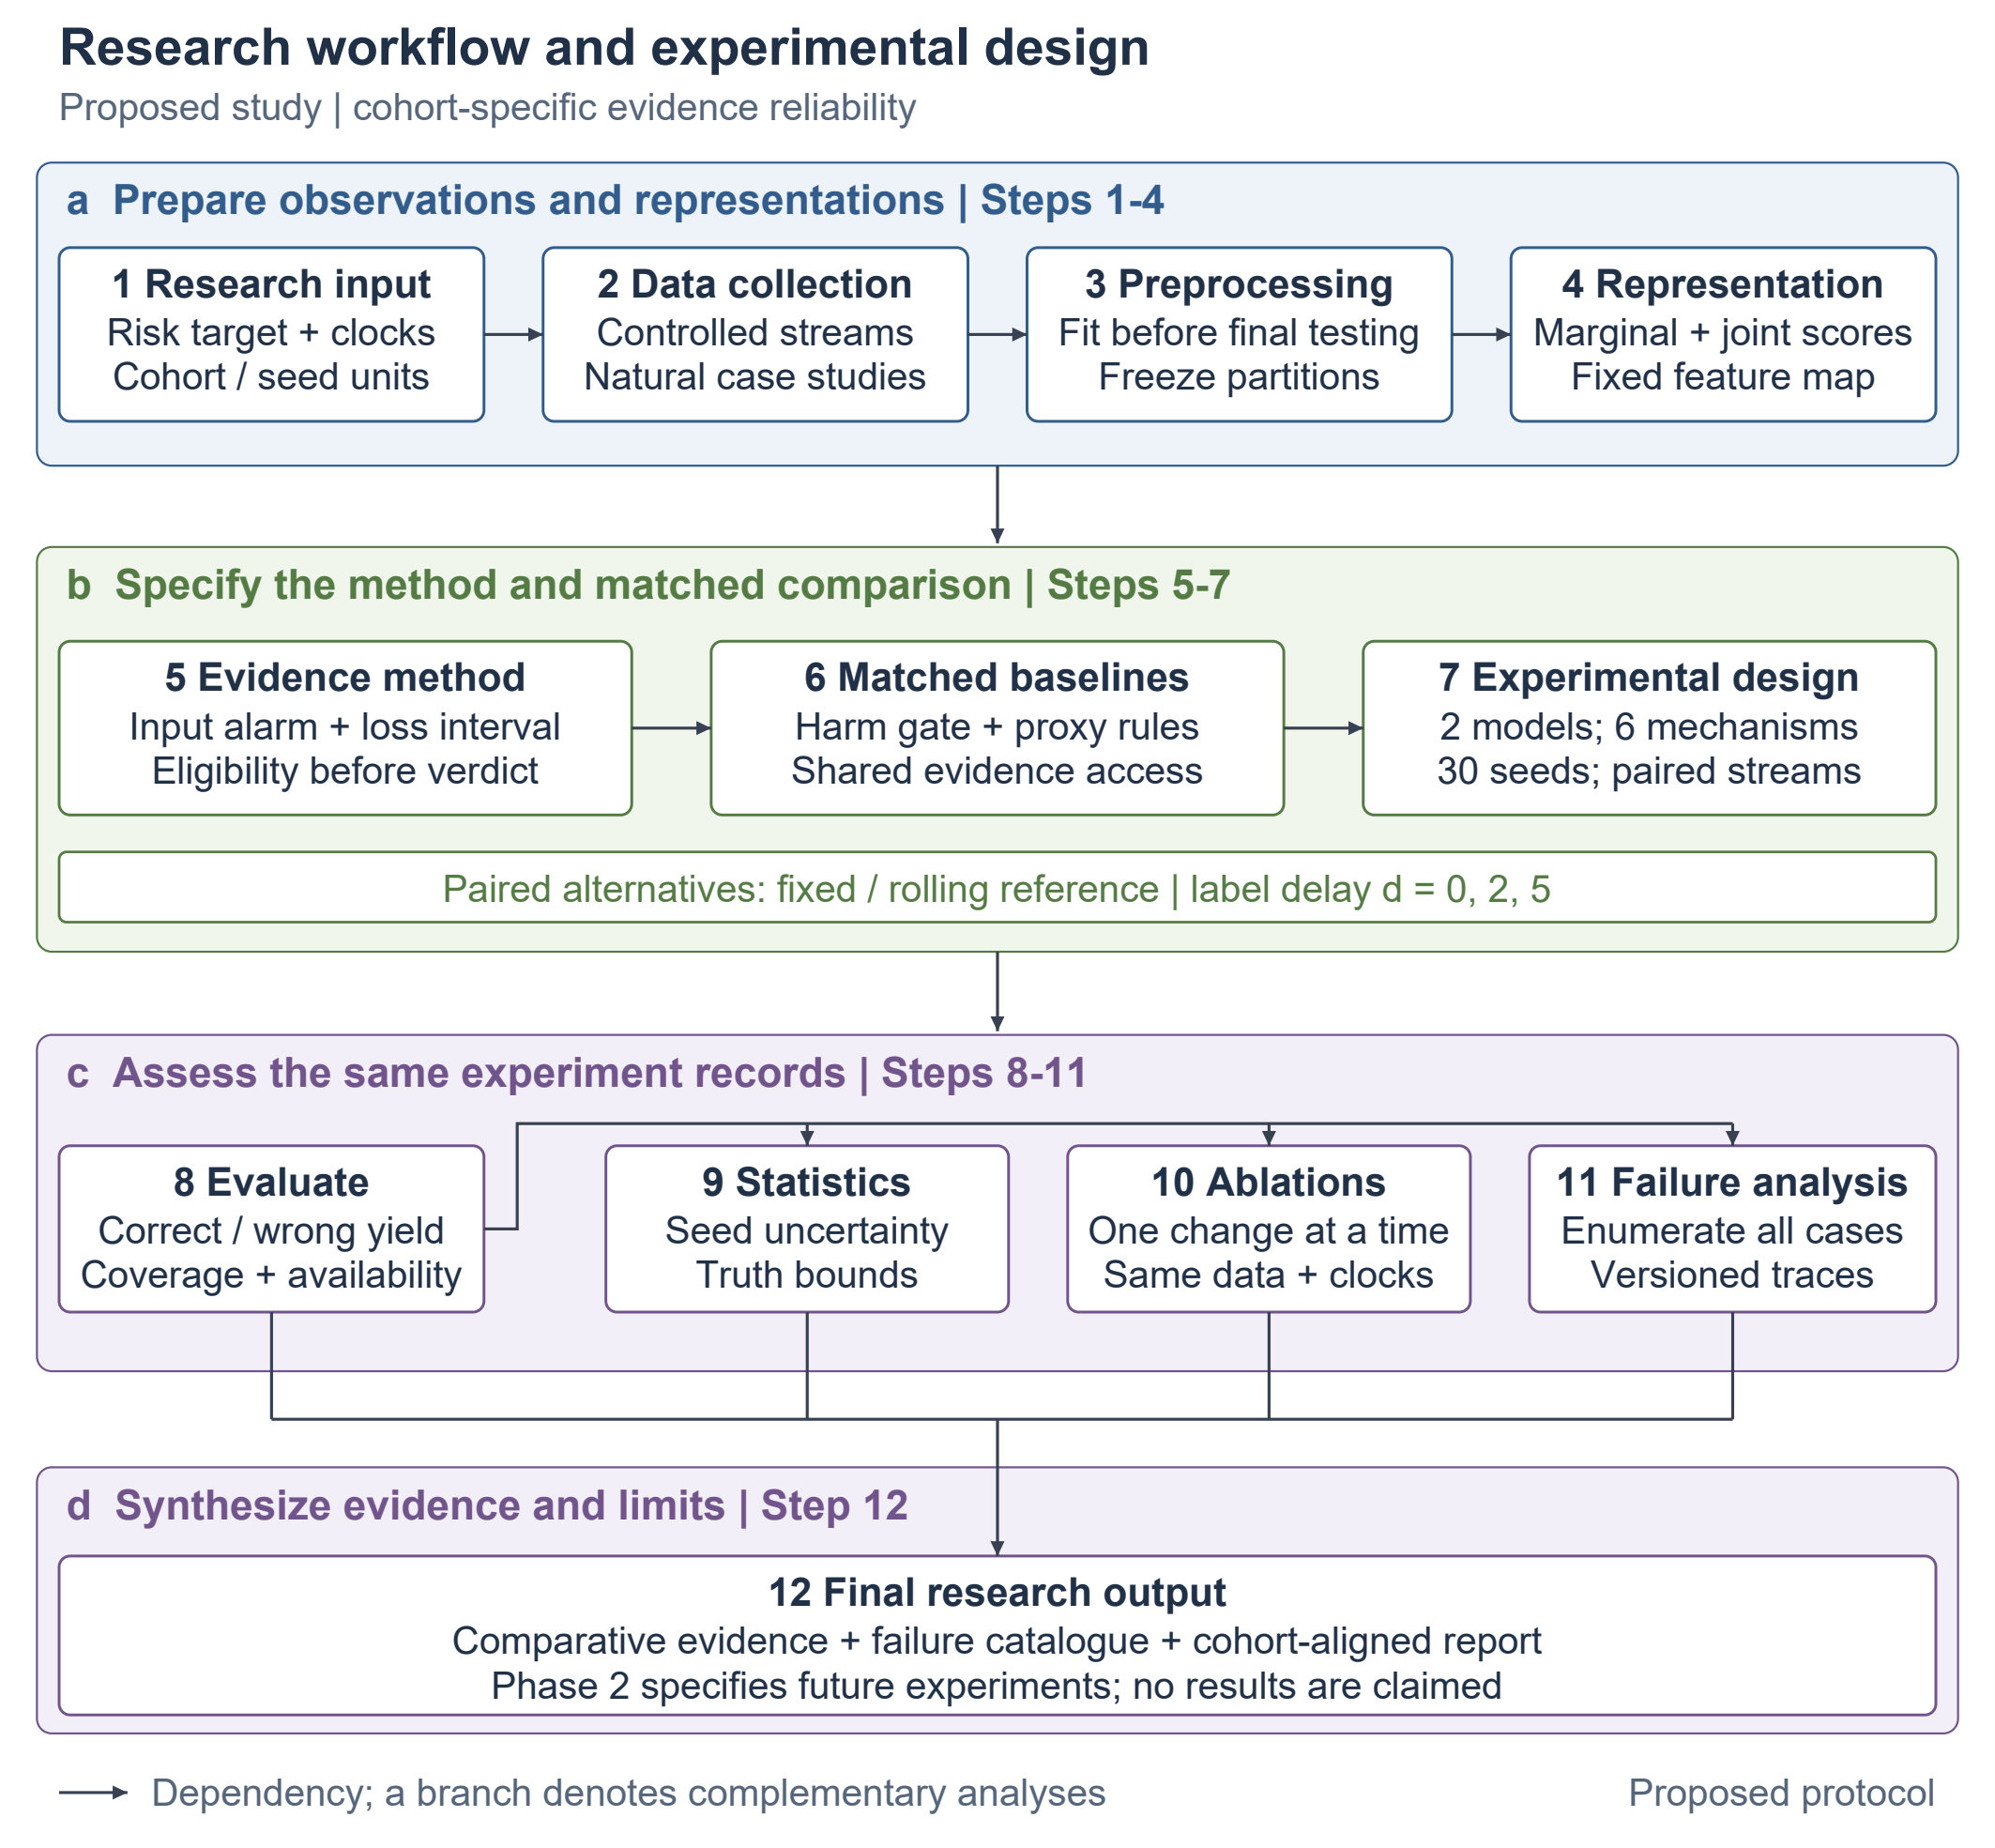
\includegraphics{../../research_figures/methodology_overview.png}
\caption{Figure 1. Proposed methodology overview.}
\end{figure}

\textbf{Figure 1. Proposed methodology overview.} The three bands map
Steps 1--4 (data and preparation), Steps 5--7 (matched experimental
design), and Steps 8--12 (evaluation and research synthesis). Dashed
boxes denote alternative experimental settings, not sequential
operations. The figure shows the fixed and rolling input references, the
label-delay levels, the six controlled mechanisms, the two frozen
classifiers, and the 30 final seeds.

\begin{figure}
\centering
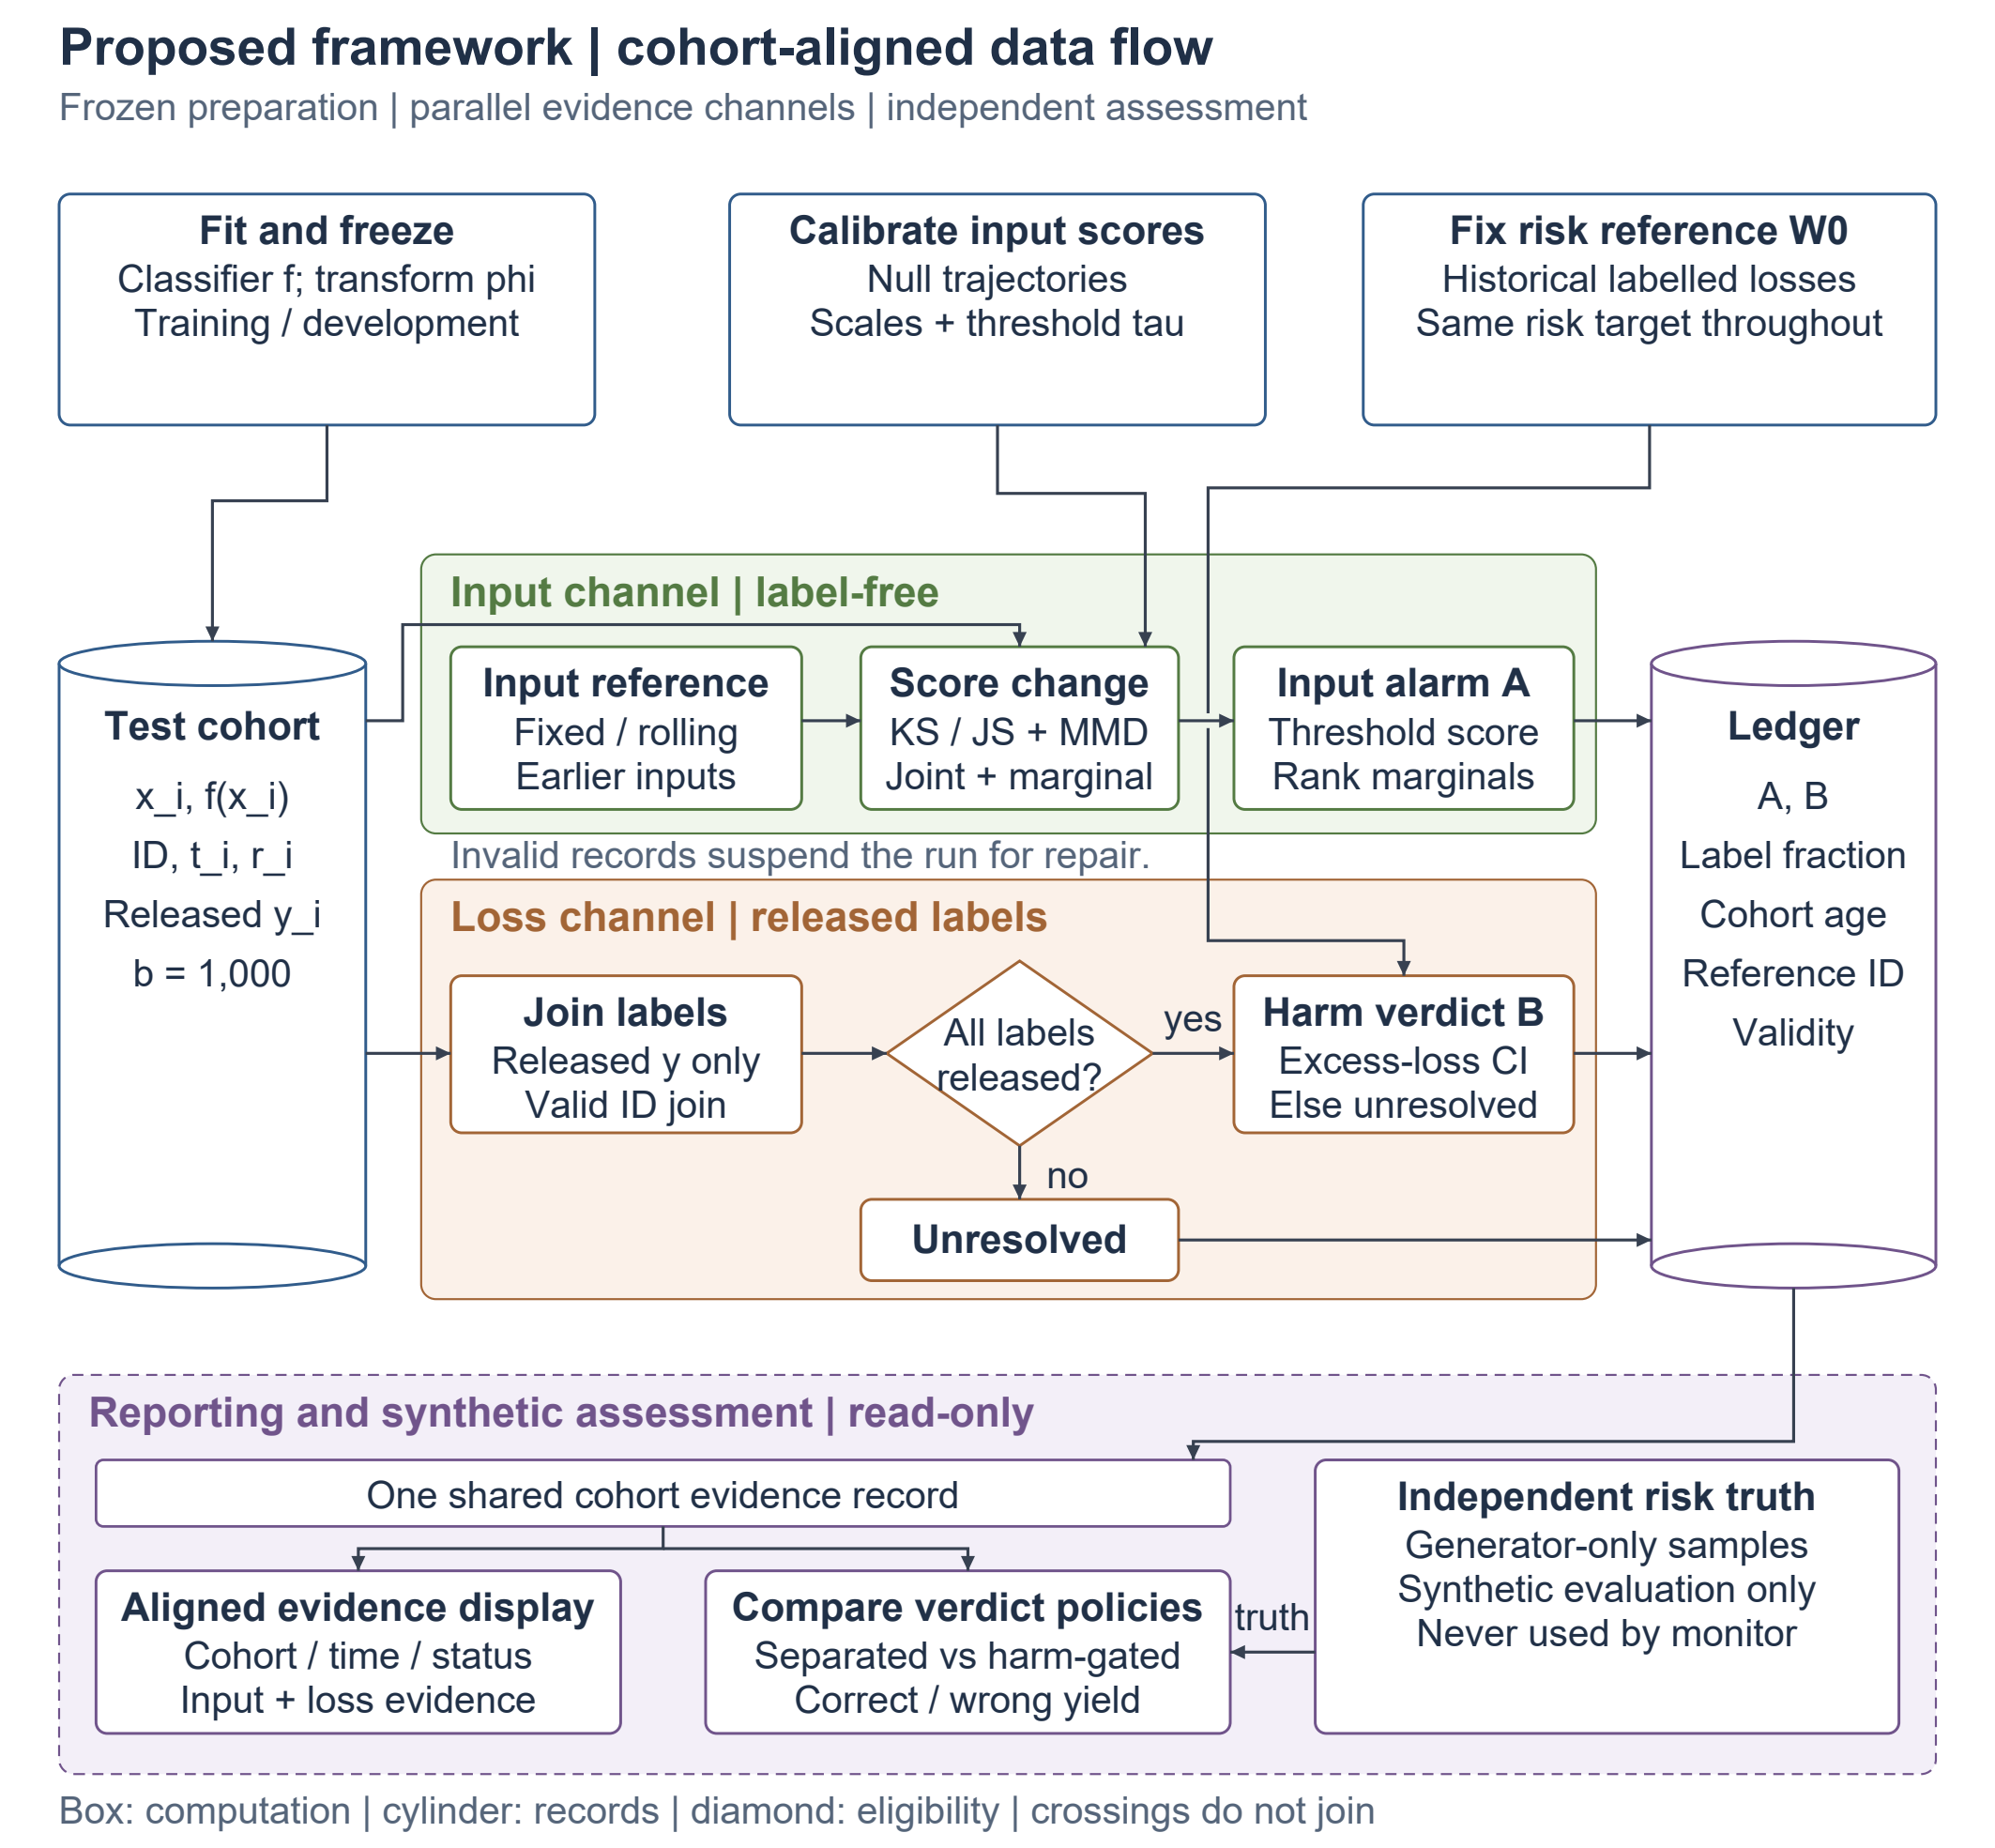
\includegraphics{../../research_figures/proposed_framework_architecture.png}
\caption{Figure 2. Proposed evidence-separated framework architecture.}
\end{figure}

\textbf{Figure 2. Proposed evidence-separated framework architecture.}
The upper band shows offline fitting and calibration: preprocessing and
frozen classifiers, input calibration banks, and a fixed predictive-risk
reference. The middle band shows two parallel, cohort-aligned channels.
The input channel compares the current cohort with a fixed or rolling
reference and produces the alarm \(A_s\) plus screened marginal
features. The label channel joins released labels by prediction ID,
computes the excess-loss interval against the fixed reference, and
produces the verdict \(B_s\). The lower band shows the aligned evidence
display and the independent evaluation. Oracle truth is hidden from the
monitor; natural-case intervals remain exploratory.

\textbf{Reading the diagrams against the twelve steps.} Figure 1 is the
reader's map: the first band corresponds to Steps 1--4, the second to
Steps 5--7, and the third to Steps 8--12. Figure 2 is the technical
expansion of Steps 1--5 and 8: it shows where calibration, input
scoring, label joining, interval construction, verdict assignment, and
evaluation truth enter the pipeline. The figures do not add adaptive
feedback loops because the proposed study freezes the classifier. A
future adaptation study would add a separate update path with its own
budget and evaluation.

\begin{center}\rule{0.5\linewidth}{0.5pt}\end{center}

\hypertarget{reproducibility-ethics-and-risk-management}{%
\subsection{6. Reproducibility, Ethics, and Risk
Management}\label{reproducibility-ethics-and-risk-management}}

\textbf{Data ethics.} The study uses public benchmark datasets and a
synthetic generator. It does not involve human participants, personal
data, or clinical records. Electricity, NOAA Weather, and Covertype are
public sources; their licences and redistribution conditions will be
recorded in the data cards. Synthetic data are generated from declared
distributions and contain no personal information. If a future extension
uses medical images or analyst participants, it will require separate
ethics review.

\textbf{Reproducibility.} The protocol manifest freezes seeds, dataset
hashes, split indices, event schedules, parameter grids, solver
settings, calibration banks, thresholds, metric denominators, and
analysis scripts. The code and environment will be versioned. The report
will distinguish development runs from final runs and will retain
failure logs. Reused input scores and regime-risk estimates will avoid
repeating identical calculations for label delays. A resource manifest
will state hardware, library versions, and elapsed-time limits. The
documentation and validity principles are consistent with the NIST AI
Risk Management Framework (NIST, 2023), but this study does not claim
certification or production validation.

\textbf{Table 20. Risk register.}

\begin{longtable}[]{@{}
  >{\raggedright\arraybackslash}p{(\columnwidth - 6\tabcolsep) * \real{0.25}}
  >{\raggedright\arraybackslash}p{(\columnwidth - 6\tabcolsep) * \real{0.25}}
  >{\raggedright\arraybackslash}p{(\columnwidth - 6\tabcolsep) * \real{0.25}}
  >{\raggedright\arraybackslash}p{(\columnwidth - 6\tabcolsep) * \real{0.25}}@{}}
\toprule
Risk & Likelihood & Impact & Mitigation \\
\midrule
\endhead
A workshop or CCIS paper is judged ineligible under a strict Q1--Q2
reading & Medium & High & Keep the eligibility audit visible; if
required, replace S4--S7 with full papers from Q1 journals \\
Thirty seeds give wide intervals & High & Medium & Report finite-sample
and bootstrap uncertainty; label precision-limited comparisons as
inconclusive \\
Natural streams lack certified harm truth & High & Medium & Keep natural
results descriptive; do not assign synthetic \(I\), FR, or FH \\
Calibration banks are computationally expensive & Medium & Medium &
Reuse banks across classifiers and delays; report calibration cost
separately \\
Reference policy is confounded with cohort composition & Medium & High &
Apply both policies to the same realised stream; keep the harm reference
fixed \\
Label delay is modelled as constant and complete & Medium & Medium &
State the limitation; treat selective and permanent missingness as
future work \\
Display implies more certainty than the analysis supports & Medium &
High & Use interval, coverage, and evidence-age encodings; test internal
consistency; avoid causal language \\
Scope creep into image, adaptation, or analyst studies & Medium & High &
Keep the Phase 2 scope explicit; defer those questions to separate
studies \\
\bottomrule
\end{longtable}

\begin{center}\rule{0.5\linewidth}{0.5pt}\end{center}

\hypertarget{conclusion}{%
\subsection{7. Conclusion}\label{conclusion}}

Phase 2 has extended the Phase 1 review with eight additional 2025--2026
studies and has developed a methodology for evaluating evidence
reliability in explainable data-drift monitoring. The review shows that
detection benchmarks, window-dependent interpretation, label-based
uncertainty, explanation-triggered retraining, and feedback detection
answer different questions. Their scores cannot be treated as
interchangeable measures of harm.

The refined gap is specific: for frozen tabular classifiers, no reviewed
protocol jointly isolates fixed versus rolling input references, one
invariant excess-risk target, independently bounded harm truth, and
matched gated versus non-gated decisions at delayed checkpoints. The
proposed methodology addresses this gap by separating input evidence
from released-label loss evidence, freezing the classifier, declaring
label-release times, and evaluating verdict correctness and coverage
rather than detection accuracy alone.

The study is an evaluation contribution. It does not claim a new
detector, a completed implementation, a measured improvement, analyst
benefit, or adaptation benefit. Its value lies in making the evidential
limits of drift monitoring testable: an alarm is not harm, a reference
choice changes the question, and a delayed label is not current
evidence. The methodology diagrams and the evidence-separated display
translate those limits into a reproducible protocol and a visual design
that can be evaluated in subsequent work.

\begin{center}\rule{0.5\linewidth}{0.5pt}\end{center}

\hypertarget{references}{%
\subsection{References}\label{references}}

Alencar, B., Cassales, G., Gomes, H. M., Prazeres, C., Rios, T., Bifet,
A., \& Rios, R. (2026). Concept drift detection in delayed and partially
labeled data streams: An experimental survey. \emph{Digital Signal
Processing, 182}, 106325.

Assis, D. N., \& Souza, V. M. A. (2025). ADWIN-U: Adaptive windowing for
unsupervised drift detection on data streams. \emph{Knowledge and
Information Systems, 67}(11), 10005--10034.

Bayram, F., Ahmed, B. S., \& Kassler, A. (2022). From concept drift to
model degradation: An overview on performance-aware drift detectors.
\emph{Knowledge-Based Systems, 245}, 108632.

Cerqueira, V., Gomes, H. M., Heyden, M., Pfahringer, B., \& Bifet, A.
(2026). A framework for evaluating and benchmarking concept drift
detection methods. In \emph{Proceedings of the 32nd ACM SIGKDD
Conference on Knowledge Discovery and Data Mining} (pp.~8671--8682).
ACM.

Eliades, C., \& Papadopoulos, H. (2025). A conformal martingales
approach for recurrent concept drift. In \emph{Proceedings of COPA 2025}
(PMLR 266, pp.~706--724).

El-Yaniv, R., \& Wiener, Y. (2010). On the foundations of noise-free
selective classification. \emph{Journal of Machine Learning Research,
11}, 1605--1641.

Gălmeanu, H., \& Andonie, R. (2024). Concept drift visualization of SVM
with shifting window. \emph{arXiv:2406.13754}.

Gower-Winter, B., Groen, M., \& Krempl, G. (2026). The window dilemma:
Why concept drift detection is ill-posed. In \emph{Advances in
Intelligent Data Analysis XXIV} (LNCS 16513, pp.~371--384). Springer.

Gower-Winter, B., Krempl, G., Dragomiretskiy, S., Jelsma, T., \& Siebes,
A. (2025). Identifying predictions that influence the future: Detecting
performative concept drift in data streams. \emph{Proceedings of the
AAAI Conference on Artificial Intelligence, 39}(11), 11726--11734.

Greco, S., Vacchetti, B., Apiletti, D., \& Cerquitelli, T. (2025).
Unsupervised concept drift detection from deep learning representations
in real-time. \emph{IEEE Transactions on Knowledge and Data Engineering,
37}(10), 6232--6245.

Gretton, A., Borgwardt, K. M., Rasch, M. J., Schölkopf, B., \& Smola, A.
(2012). A kernel two-sample test. \emph{Journal of Machine Learning
Research, 13}, 723--773.

Guerrero Cano, J. V., Aguiar, G. J., \& Cano, A. (2026). Anticipating to
change: A proactive approach for concept drift adaptation in data
streams. \emph{Machine Learning, 115}, Article 3.

Hinder, F., Vaquet, V., Brinkrolf, J., \& Hammer, B. (2023). Model-based
explanations of concept drift. \emph{Neurocomputing, 555}, 126640.

Hinder, F., Vaquet, V., \& Hammer, B. (2024). One or two things we know
about concept drift---a survey on monitoring in evolving environments.
Part B: Locating and explaining concept drift. \emph{Frontiers in
Artificial Intelligence, 7}, 1330258.

Hoeffding, W. (1963). Probability inequalities for sums of bounded
random variables. \emph{Journal of the American Statistical Association,
58}(301), 13--30.

Holm, S. (1979). A simple sequentially rejective multiple test
procedure. \emph{Scandinavian Journal of Statistics, 6}(2), 65--70.

Komnick, D., Lammers, K., Hammer, B., Vaquet, V., \& Hinder, F. (2026).
Causal explanation of concept drift---A truly actionable approach. In
\emph{Machine Learning and Principles and Practice of Knowledge
Discovery in Databases: ECML PKDD 2025 Workshops} (CCIS 2842,
pp.~396--412). Springer.

Kraus, A., \& van der Aa, H. (2025). Machine learning-based detection of
concept drift in business processes. \emph{Process Science, 2}, Article
5.

Künsch, H. R. (1989). The jackknife and the bootstrap for general
stationary observations. \emph{Annals of Statistics, 17}(3), 1217--1241.

Lu, P., Lu, J., Liu, A., \& Zhang, G. (2025). Early concept drift
detection via prediction uncertainty. \emph{Proceedings of the AAAI
Conference on Artificial Intelligence, 39}(18), 19124--19132.

Lukats, D., Zielinski, O., Hahn, A., \& Stahl, F. (2025). A benchmark
and survey of fully unsupervised concept drift detectors on real-world
data streams. \emph{International Journal of Data Science and Analytics,
19}, 1--31.

National Institute of Standards and Technology. (2023). \emph{Artificial
Intelligence Risk Management Framework (AI RMF 1.0)} (NIST AI 100-1).

Roschewitz, M., Mehta, R., Jones, C., \& Glocker, B. (2025). Automatic
dataset shift identification to support safe deployment of medical
imaging AI. In \emph{MICCAI 2025} (LNCS 15966, pp.~67--76). Springer.

Souza, V. M. A., dos Reis, D. M., Maletzke, A. G., \& Batista, G. E. A.
P. A. (2020). Challenges in benchmarking stream learning algorithms with
real-world data. \emph{Data Mining and Knowledge Discovery, 34},
1805--1858.

Szűcs, G., \& Németh, M. (2025). Domino drift effect approach for
probability estimation of feature drift in high-dimensional data.
\emph{Knowledge and Information Systems, 67}, 4597--4621.

Tan, N., Shih, Y.-C., Yang, D., \& Salunkhe, A. (2025). Flexible and
efficient drift detection without labels. In \emph{2025 IEEE
International Conference on Data Mining Workshops} (pp.~265--274). IEEE.

Teixeira, B., Pinto, T., \& Vale, Z. (2025). Detecting concept drift
with SHapley Additive ExPlanations for intelligent model retraining in
energy generation forecasting. In \emph{Explainable Artificial
Intelligence (xAI)} (CCIS 2577, pp.~156--168). Springer.

Tran, Q.-T., Le-Khac, N.-A., \& Bertolotto, M. (2026). Concept drift
detection in image data stream: A survey on current literature,
limitations and future directions. \emph{Artificial Intelligence Review,
59}, Article 33.

Wang, X., Chen, W., Xia, J., Chen, Z., Xu, D., Wu, X., Xu, M., \&
Schreck, T. (2020). ConceptExplorer: Visual analysis of concept drifts
in multi-source time-series data. In \emph{2020 IEEE Conference on
Visual Analytics Science and Technology} (pp.~1--11). IEEE.

Yang, W., Li, Z., Liu, M., Lu, Y., Cao, K., Maciejewski, R., \& Liu, S.
(2020). Diagnosing concept drift with visual analytics. In \emph{2020
IEEE Conference on Visual Analytics Science and Technology}
(pp.~12--23). IEEE.

\begin{center}\rule{0.5\linewidth}{0.5pt}\end{center}

\hypertarget{appendix-a-phase-2-compliance-checklist}{%
\subsection{Appendix A --- Phase 2 Compliance
Checklist}\label{appendix-a-phase-2-compliance-checklist}}

\textbf{Table A1. Requirement-to-section mapping.}

\begin{longtable}[]{@{}
  >{\raggedright\arraybackslash}p{(\columnwidth - 4\tabcolsep) * \real{0.33}}
  >{\raggedright\arraybackslash}p{(\columnwidth - 4\tabcolsep) * \real{0.33}}
  >{\raggedright\arraybackslash}p{(\columnwidth - 4\tabcolsep) * \real{0.33}}@{}}
\toprule
Requirement & Where addressed & Status \\
\midrule
\endhead
Move from literature and gaps to a justified methodology & Sections 1--4
& Complete \\
Extend the Phase 1 review & Sections 1.1, 2.1 & Complete \\
Select 8--10 additional papers & Section 2.1; Table 1 (S1--S8) &
Complete: eight additions \\
Published 2025--2026 & Table 1 & Complete \\
Original research, not editorial, opinion, news, or webpage & Section
2.1; Table 1 & Complete \\
Q1--Q2 journal, conference paper, or book chapter & Table 1; Appendix B
& Complete under the conference/book-chapter route; see residual note \\
Direct relevance & Sections 2.2--2.3 & Complete \\
Identifiable method, setup, or framework & Table 2 & Complete \\
Sufficient dataset, method, and evaluation detail & Tables 2--4 &
Complete \\
Reputable publisher & Table 1 & ACM, IEEE, AAAI, Springer, PMLR \\
Three-paper comparison table with all nine columns & Table 4 &
Complete \\
Synthesised, not copied & Sections 2.2--2.4 & Complete \\
At least three research gaps & Section 3.1; Table 5 & Complete:
G1--G3 \\
Gap matrix with evidence from Paper 1, 2, 3 and opportunity & Table 5 &
Complete \\
What has already been done & Section 3.2 & Complete \\
What approaches currently exist & Section 3.2 & Complete \\
What their limitations are & Section 3.2 & Complete \\
What remains insufficiently investigated & Section 3.2 & Complete \\
Why the gap is important & Section 3.2 & Complete \\
How the research will address it & Sections 3.2--3.4 & Complete \\
Step 1 --- Define the Research Input & Section 4, Step 1 & Complete \\
Step 2 --- Data Collection & Section 4, Step 2 & Complete \\
Step 3 --- Data Preprocessing & Section 4, Step 3 & Complete \\
Step 4 --- Feature Engineering / Representation & Section 4, Step 4 &
Complete \\
Step 5 --- Proposed Model / Method & Section 4, Step 5 & Complete \\
Step 6 --- Baseline Methods & Section 4, Step 6 & Complete \\
Step 7 --- Experimental Design & Section 4, Step 7 & Complete \\
Step 8 --- Evaluation Metrics & Section 4, Step 8 & Complete \\
Step 9 --- Statistical / Comparative Analysis & Section 4, Step 9 &
Complete \\
Step 10 --- Ablation and Component Analysis & Section 4, Step 10 &
Complete \\
Step 11 --- Error / Failure Analysis & Section 4, Step 11 & Complete \\
Step 12 --- Final Research Output & Section 4, Step 12 & Complete \\
Research methodology architecture diagram & Section 5; Figures 1--2 &
Complete: two diagrams \\
Deliverable 1 --- Extended Literature Review & Section 2 & Complete \\
Deliverable 2 --- Refined Research Gap & Section 3 & Complete \\
Deliverable 3 --- Proposed Research Methodology & Section 4 &
Complete \\
Deliverable 4 --- Research Methodology Diagram & Section 5 & Complete \\
Academic tone and references & Throughout; References & Complete \\
Proposed work only, no claimed results & Scope box; Sections 4--7 &
Complete \\
\bottomrule
\end{longtable}

\textbf{Residual compliance note.} The brief permits Q1--Q2 journal
articles, conference papers, and book chapters. The eight additions use
the conference-paper and book-chapter routes. S1 (ACM KDD), S2 (Springer
LNCS/IDA), S3 (AAAI), and S8 (AAAI) are full archival papers. S4 (IEEE
ICDMW), S5--S6 (Springer CCIS), and S7 (PMLR/COPA) are peer-reviewed
workshop or chapter routes. If the instructor interprets the Q1--Q2
requirement as applying to every selected item, S4--S7 should be
replaced by full papers from Q1 journals. This is an administrative
eligibility decision, not a methodological one.

\begin{center}\rule{0.5\linewidth}{0.5pt}\end{center}

\hypertarget{appendix-b-venue-eligibility-notes}{%
\subsection{Appendix B --- Venue Eligibility
Notes}\label{appendix-b-venue-eligibility-notes}}

\textbf{Table B1. Venue route and evidence for each additional study.}

\begin{longtable}[]{@{}
  >{\raggedright\arraybackslash}p{(\columnwidth - 8\tabcolsep) * \real{0.20}}
  >{\raggedright\arraybackslash}p{(\columnwidth - 8\tabcolsep) * \real{0.20}}
  >{\raggedright\arraybackslash}p{(\columnwidth - 8\tabcolsep) * \real{0.20}}
  >{\raggedright\arraybackslash}p{(\columnwidth - 8\tabcolsep) * \real{0.20}}
  >{\raggedright\arraybackslash}p{(\columnwidth - 8\tabcolsep) * \real{0.20}}@{}}
\toprule
ID & Venue & Publisher & Route & Eligibility note \\
\midrule
\endhead
S1 & ACM SIGKDD Conference (KDD) & ACM & Full conference paper &
Top-tier data-mining venue; archival proceedings \\
S2 & Advances in Intelligent Data Analysis (IDA), LNCS & Springer Nature
& Research chapter & Peer-reviewed LNCS chapter; archival \\
S3 & AAAI Conference on Artificial Intelligence & AAAI & Full conference
paper & Top-tier AI venue; archival proceedings \\
S4 & IEEE International Conference on Data Mining Workshops & IEEE &
Workshop paper & Peer-reviewed IEEE workshop proceedings; not a Q1
journal \\
S5 & ECML PKDD 2025 Workshops, CCIS & Springer Nature & Research chapter
& Peer-reviewed CCIS chapter; workshop route \\
S6 & xAI Conference, CCIS & Springer Nature & Research chapter &
Peer-reviewed CCIS chapter; conference route \\
S7 & COPA 2025, PMLR & PMLR & Conference paper & Peer-reviewed PMLR
proceedings; workshop/conference route \\
S8 & AAAI Conference on Artificial Intelligence & AAAI & Full conference
paper & Top-tier AI venue; archival proceedings \\
\bottomrule
\end{longtable}

\textbf{Selection rationale.} The corpus deliberately combines full
archival papers with workshop and chapter routes. The full papers
provide strong evidence about detection benchmarks, window
interpretation, uncertainty, and feedback. The workshop and chapter
papers provide the closest available evidence on label-free batching,
causal explanation, explanation-triggered retraining, and recurrent
conformal monitoring. Excluding them would improve venue prestige but
would weaken topical coverage. The report states the route explicitly
rather than implying journal quartiles for proceedings.

\textbf{What would change under a strict Q1--Q2 reading.} If every
selected paper must be a Q1--Q2 journal article, the corpus would need
to be rebuilt around journal papers on drift detection and monitoring.
That would likely exclude the causal-explanation and
conformal-recurrence studies, which are directly relevant to the gap.
The methodological design would not change, but the literature review
would lose its closest evidence on explanation and recurrence. This
trade-off should be resolved with the instructor before submission.

\begin{center}\rule{0.5\linewidth}{0.5pt}\end{center}

\emph{End of report.}

\end{document}
